% Лабораторная работа по АСиСу № 8
% Михедов Константин Константинович

% Тип документа: статья, на бумаге А4
\documentclass[a4paper]{article}

% Подключение сторонних tex файлов 
\usepackage{import}


% Основные данные - ВУЗ, факультет, город...
\import{./../../stuff/tex}{config.tex}

% Подключение необходимых зависимостей
\import{./../../stuff/tex/settings}{packages.tex}
% Настройка подключенных пакетов
\import{./../../stuff/tex/settings}{preferences.tex}


% Шаблон титульной страницы 
\import{./../../stuff/tex/templates}{title.tex}
% Упрощенный блок "выполнил"
\import{./../../stuff/tex/templates}{sign1.tex}
% Макрос для содержания
\import{./../../stuff/tex/templates}{toc.tex}

% Определяем название документа
\title{
  Лабораторная работа №9 по курсу \\
  <<Компьютерный практикум <<Администрирование систем и сетей>>  
}
% Отключаем отображение правительства
\renewcommand{\government}{}
% Отключаем сокращенное нзавание университета
\renewcommand{\subuniversity}{}
% Указываем преподавателя
\renewcommand{\shortteachername}{Степанянц В.Г.}


% Путь до внешних изображений
\graphicspath{ {./figures/}}


% Основной текст работы
\begin{document}
  \templatedtitlepage
  
  \toc
  \section{Ход работы}

  Все имена выбраны в соответсвии с 9 вариантом.

  \subsection{Настройка сети}

  Для выполнения данной работы потребуется \textit{NAT} сеть (с доступом в Интернет),
  создадим ее:

  \begin{figure}[H]
    \centering
    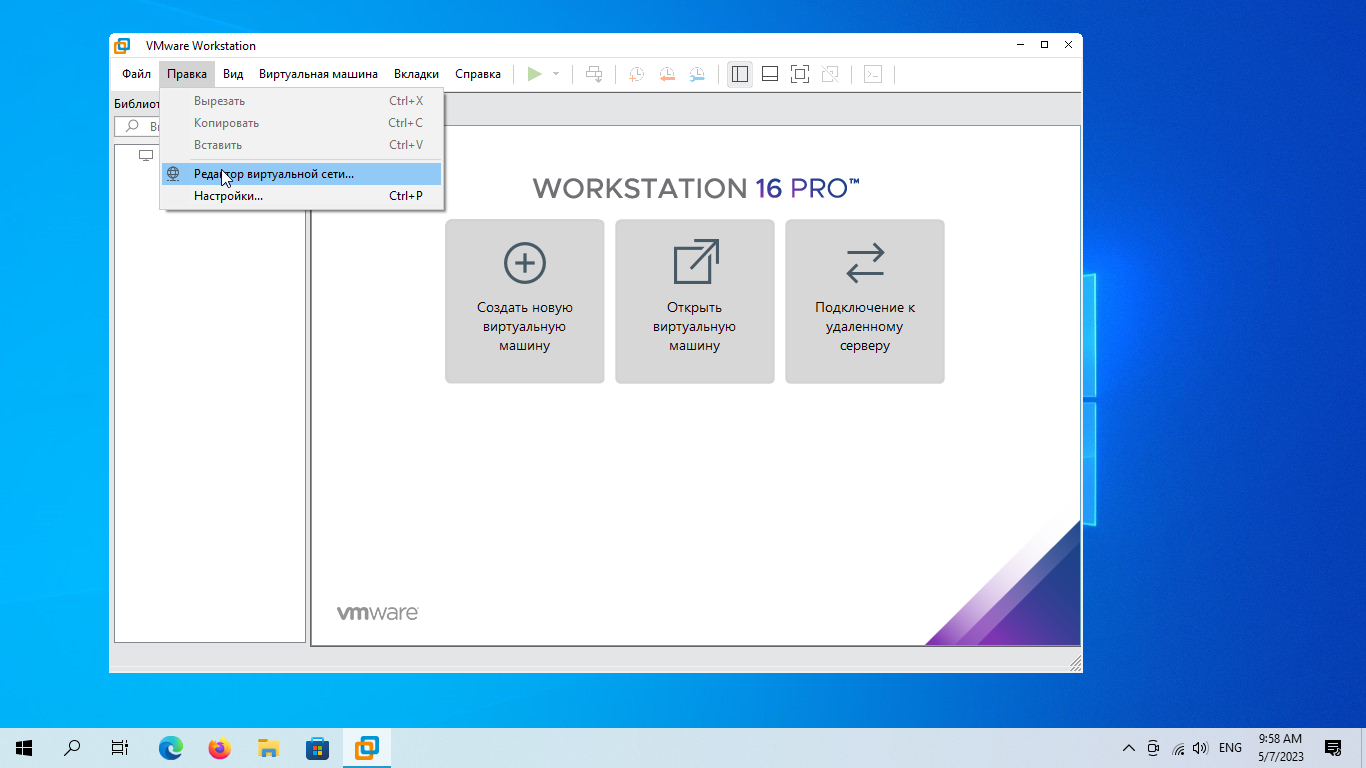
\includegraphics[width=0.85\textwidth]{9_0001}
    \caption{Открываем редактор виртуальной сети}
    \label{img:0001}
  \end{figure}

  \begin{figure}[H]
    \centering
    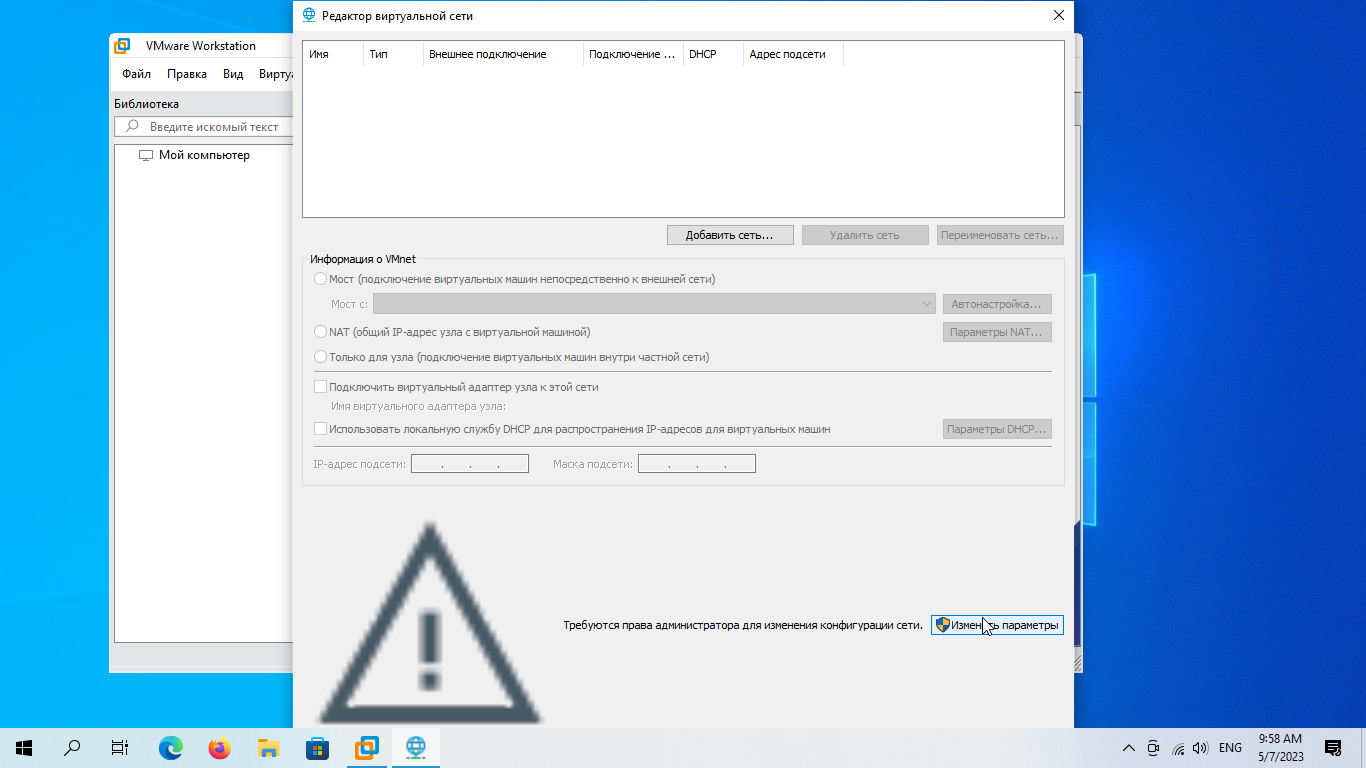
\includegraphics[width=0.85\textwidth]{9_0002}
    \caption{Разрешаем редактирование параметрова}
    \label{img:0002}
  \end{figure}

  \begin{figure}[H]
    \centering
    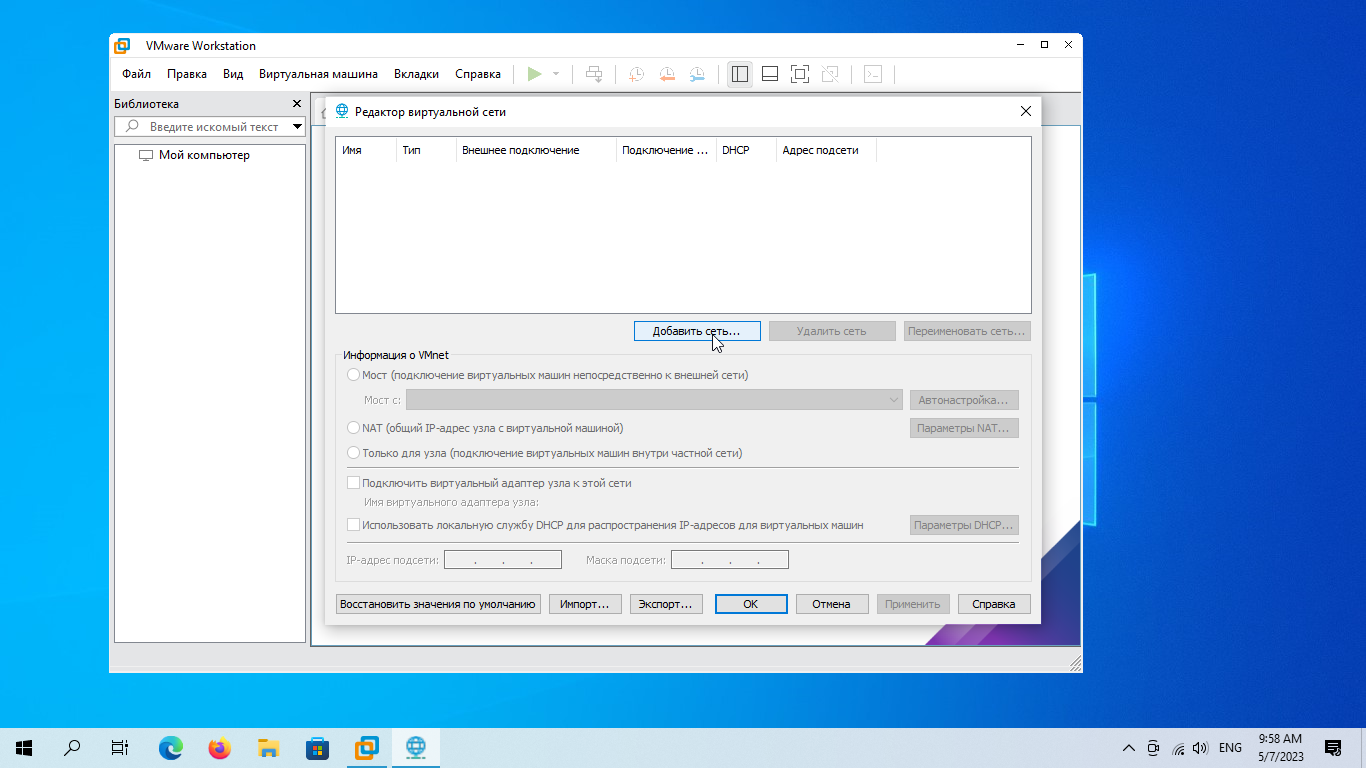
\includegraphics[width=0.85\textwidth]{9_0003}
    \caption{Добавляем новую сеть}
    \label{img:0003}
  \end{figure}

  \begin{figure}[H]
    \centering
    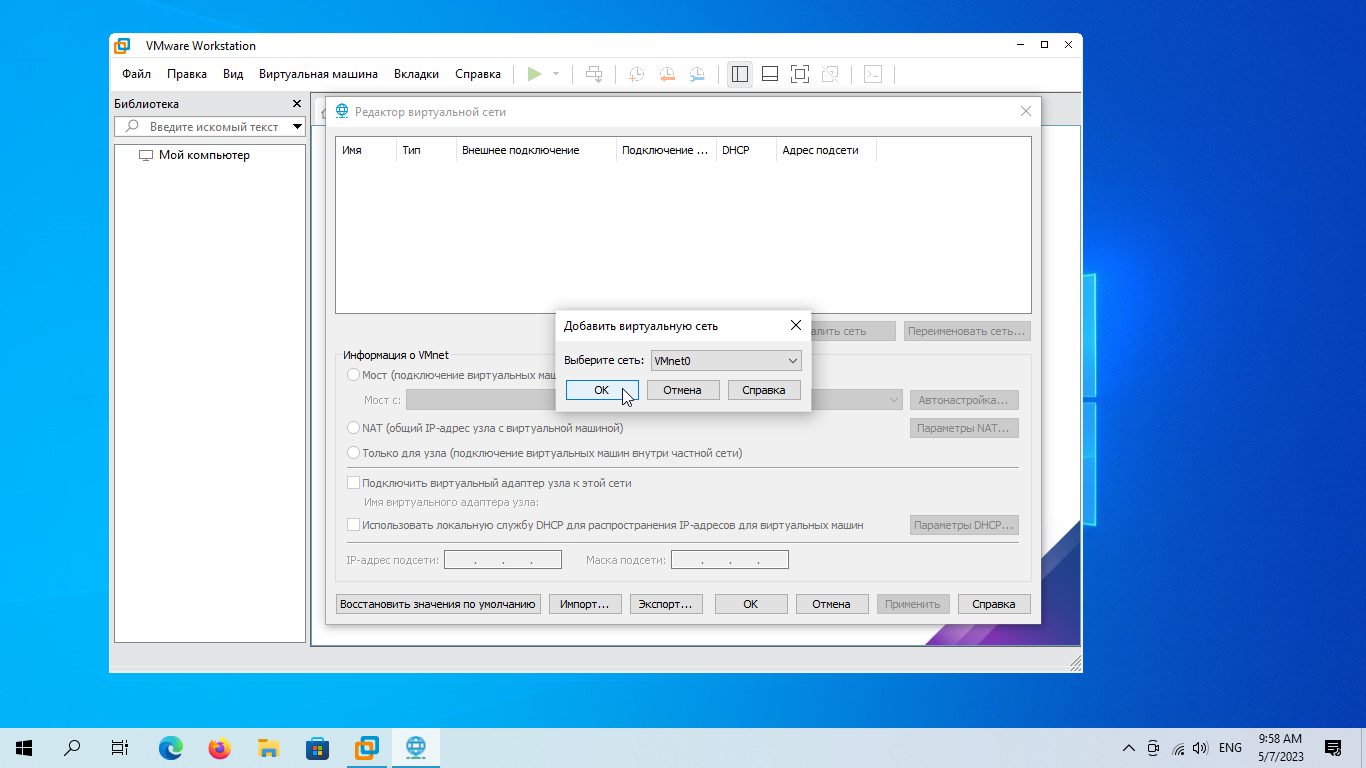
\includegraphics[width=0.85\textwidth]{9_0004}
    \caption{Выбираем для нее имя}
    \label{img:0004}
  \end{figure}

  \begin{figure}[H]
    \centering
    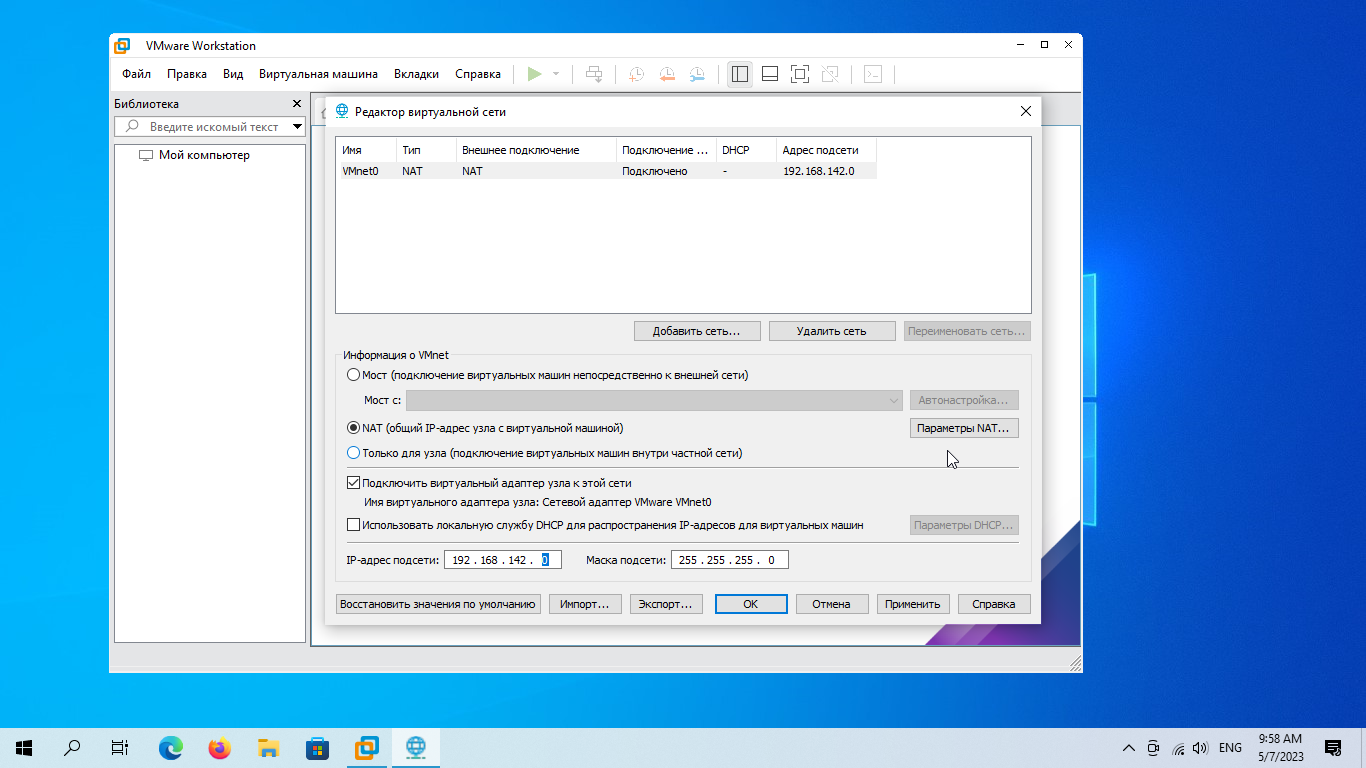
\includegraphics[width=0.85\textwidth]{9_0005}
    \caption{Устанавливаем необходимые параметры}
    \label{img:0005}
  \end{figure}

  Для новой сети необходимо указать правильные настройки, в частности ее тип - \textit{NAT},
  статус встроенного \textit{DHCP} сервера - отключен, адрес сети и маску - 192.168.142\\24
  (рис. \ref{img:0005} на стр. \pageref{img:0005}).

  \begin{figure}[H]
    \centering
    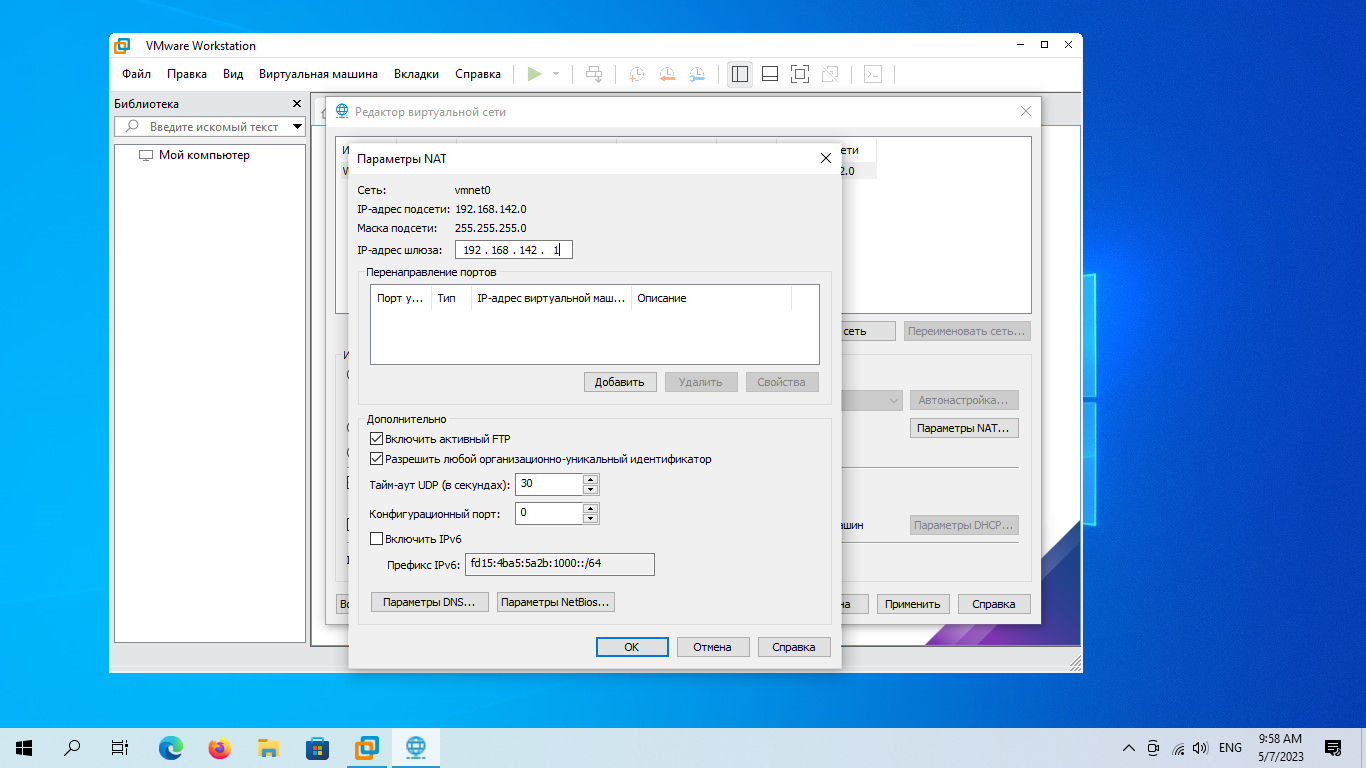
\includegraphics[width=0.85\textwidth]{9_0006}
    \caption{Параметры NAT}
    \label{img:0006}
  \end{figure}

  Также необходимо указать адрес шлюза - был выбран первый не занятый в сети 192.168.142.1.
  Через него будет осуществляться доступ в Интернет, его же можно использовать в качестве
  адреса \textit{DNS} сервера.

  \begin{figure}[H]
    \centering
    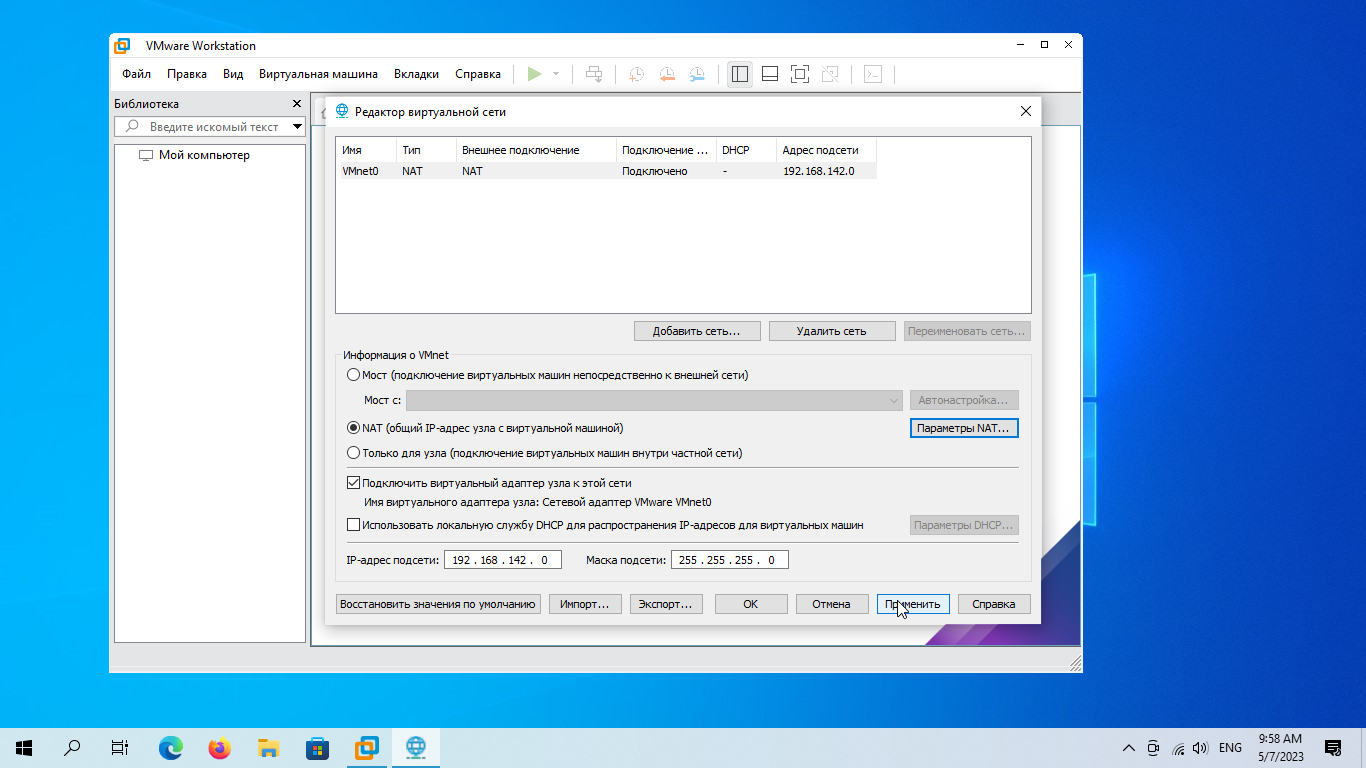
\includegraphics[width=0.85\textwidth]{9_0007}
    \caption{Применяем настройки}
    \label{img:0007}
  \end{figure}

  Сеть настроена и готова к работе.

  \subsection{Создание и настройка виртуальной машины}

  Для работы потребуется одна виртуальная машина с запущенной на ней
  Windows Server 2016. Воспользуемся заранее подготовленным образом,
  на который уже установлена данная ОС:

  \begin{figure}[H]
    \centering
    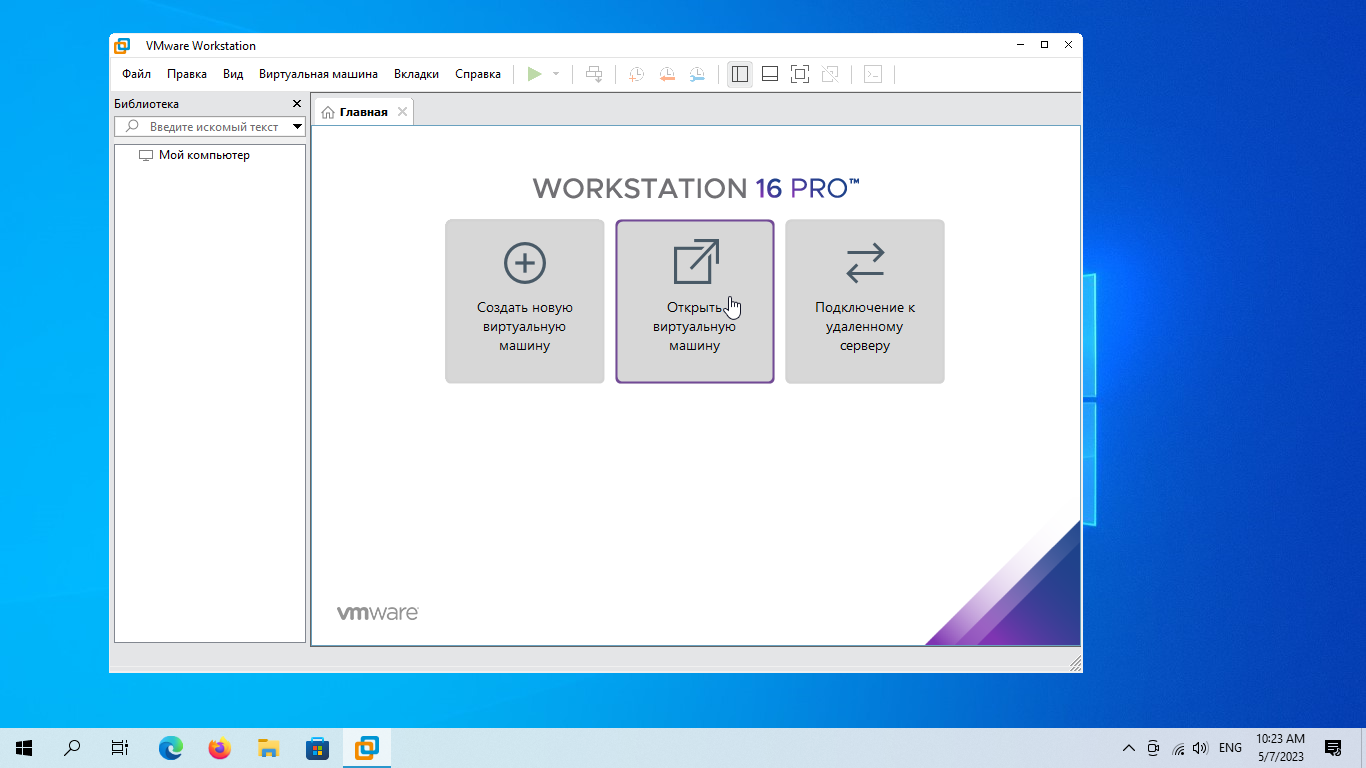
\includegraphics[width=0.85\textwidth]{9_0008}
    \caption{Начинаем импорт ВМ}
    \label{img:0008}
  \end{figure}

  \begin{figure}[H]
    \centering
    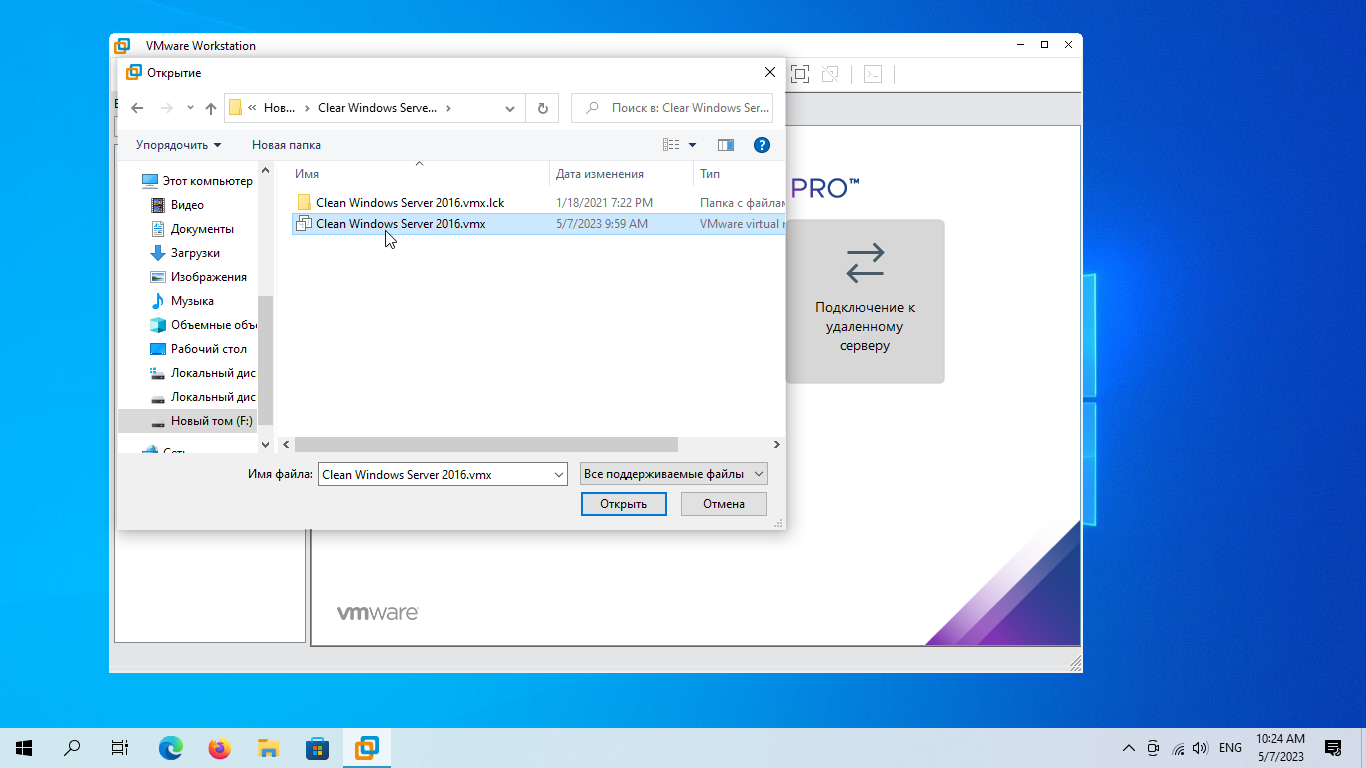
\includegraphics[width=0.85\textwidth]{9_0009}
    \caption{Указываем путь до образа}
    \label{img:0009}
  \end{figure}

  Машина создана и готова к запуску, но сначала нужно подключить ее к ранее созданной
  \textit{NAT} сети:

  \begin{figure}[H]
    \centering
    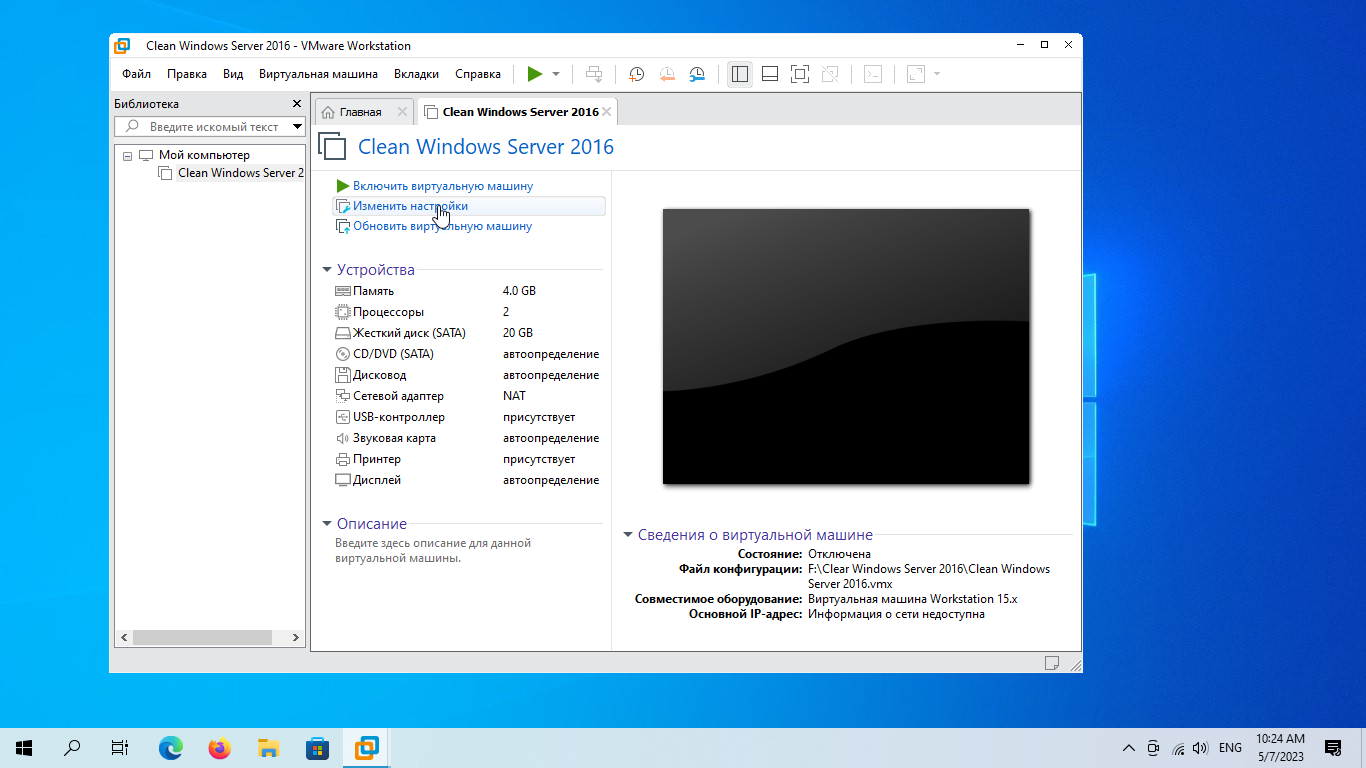
\includegraphics[width=0.85\textwidth]{9_0010}
    \caption{Открываем параметры ВМ}
    \label{img:0010}
  \end{figure}

  \begin{figure}[H]
    \centering
    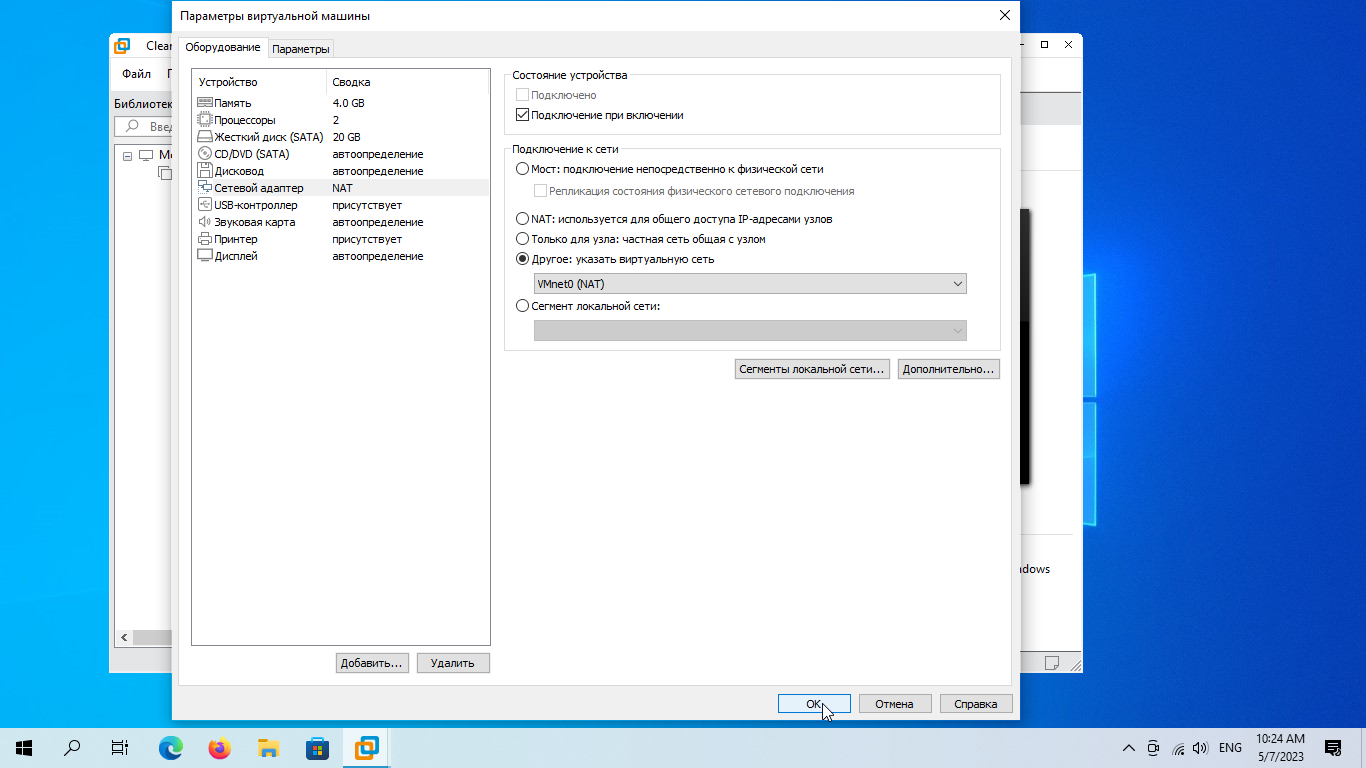
\includegraphics[width=0.85\textwidth]{9_0011}
    \caption{Подключаем сетевой адаптер к нужной сети}
    \label{img:0011}
  \end{figure}

  Теперь машина полностью настроена, запускаем:

  \begin{figure}[H]
    \centering
    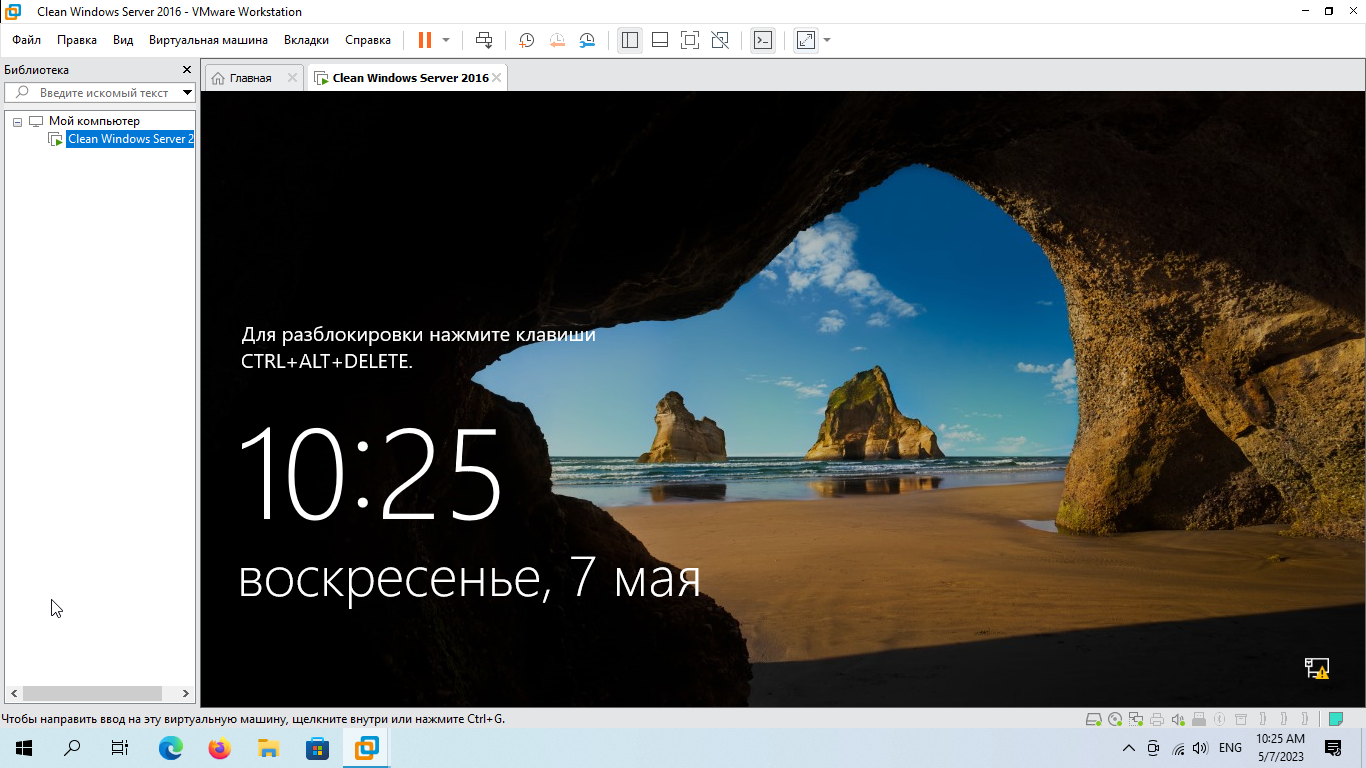
\includegraphics[width=0.85\textwidth]{9_0012}
    \caption{Запущенная ВМ}
    \label{img:0012}
  \end{figure}

  \subsection{Подготовка системы}

  Для того, чтобы перейти непосредственно к настройке \textit{DNS} сервера, сначала
  необходимо настроить сетевой адаптер, создать домен и установить необходимые компоненты. Сделаем это:

  \begin{figure}[H]
    \centering
    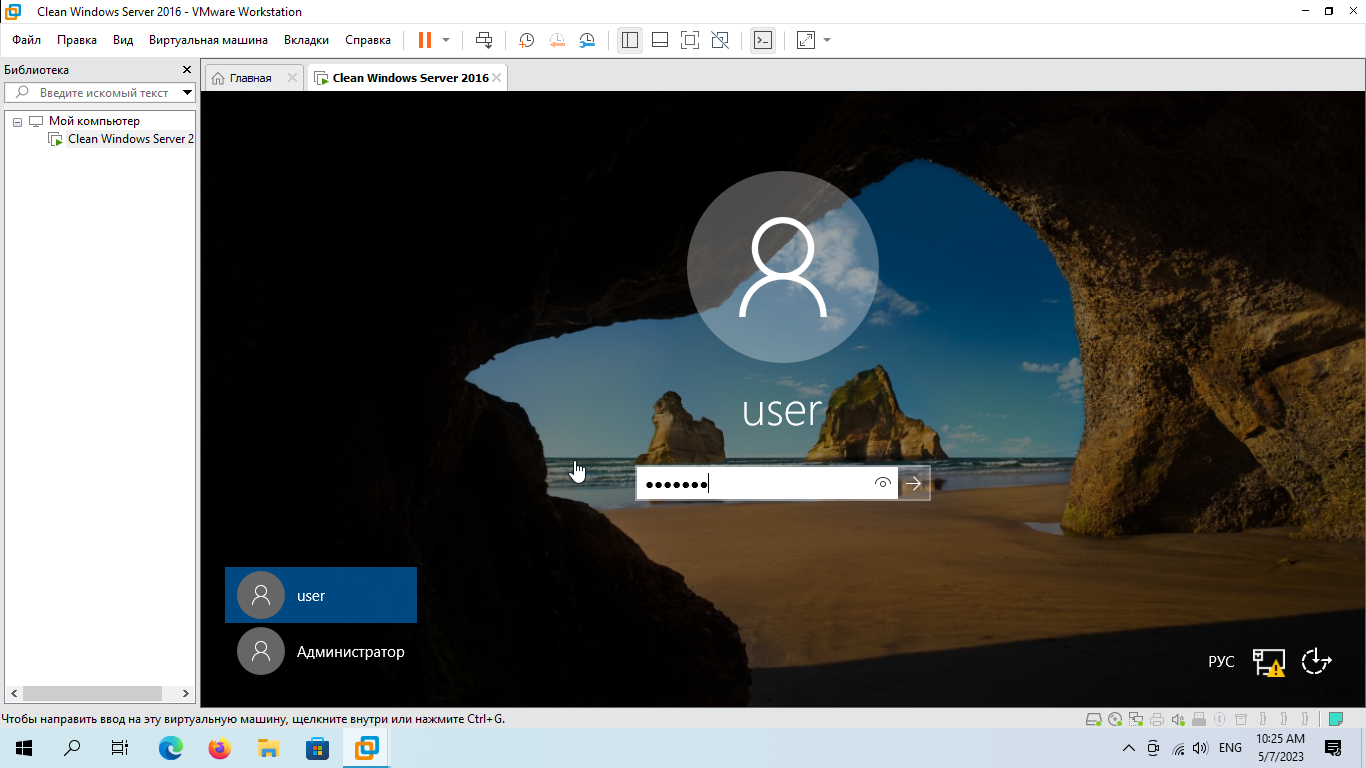
\includegraphics[width=0.85\textwidth]{9_0013}
    \caption{Входим в учетную запись пользователя}
    \label{img:0013}
  \end{figure}

  \subsubsection{Настройка сети}

  \begin{figure}[H]
    \centering
    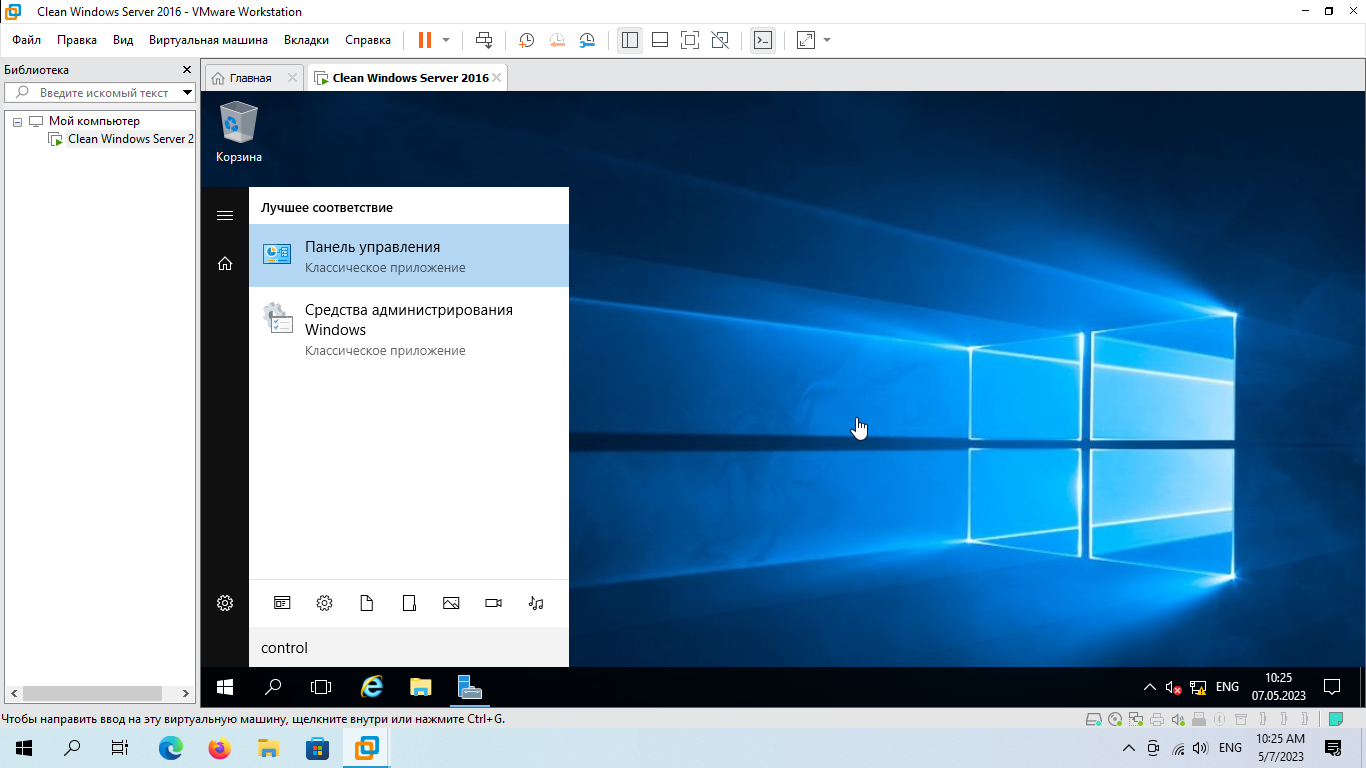
\includegraphics[width=0.85\textwidth]{9_0014}
    \caption{Открываем Панель управления}
    \label{img:0014}
  \end{figure}

  \begin{figure}[H]
    \centering
    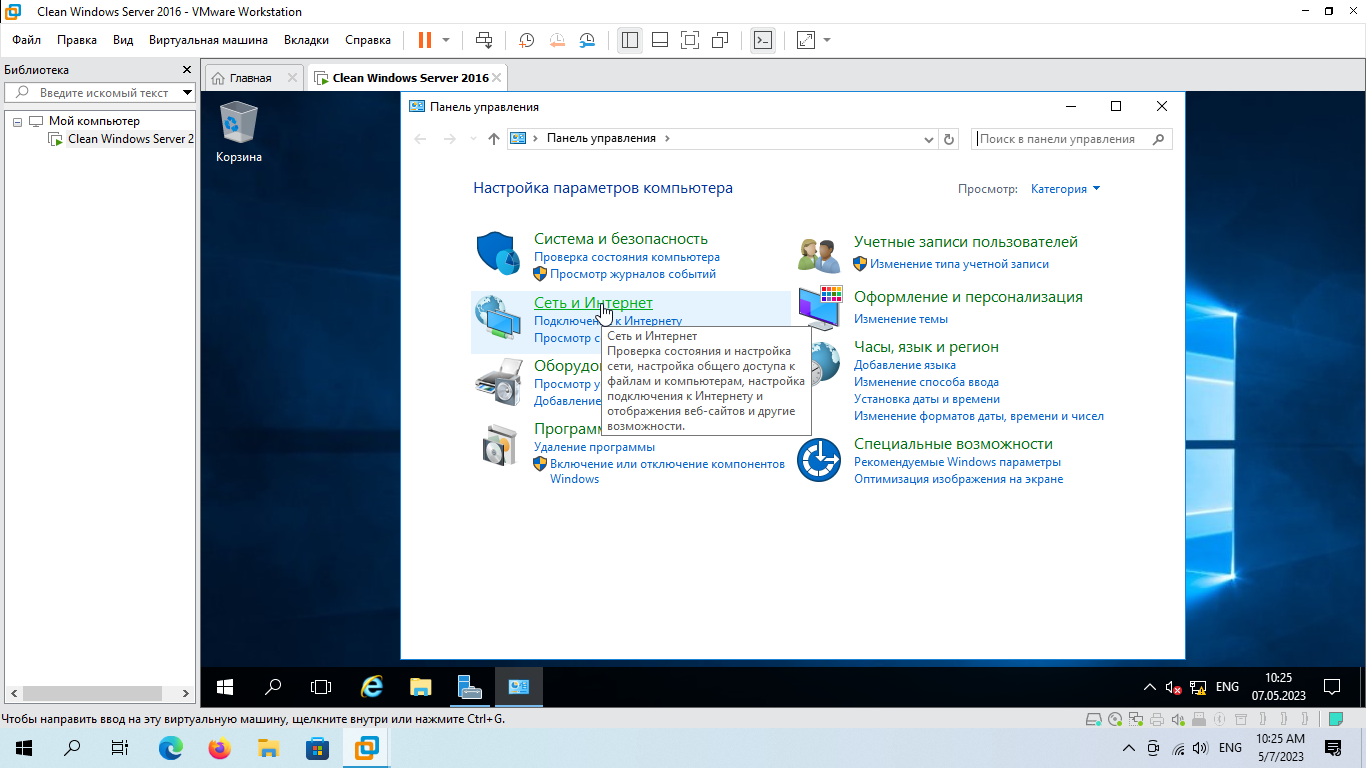
\includegraphics[width=0.85\textwidth]{9_0015}
    \caption{Переходим в пункт "Сеть и Интернет"}
    \label{img:0015}
  \end{figure}

  \begin{figure}[H]
    \centering
    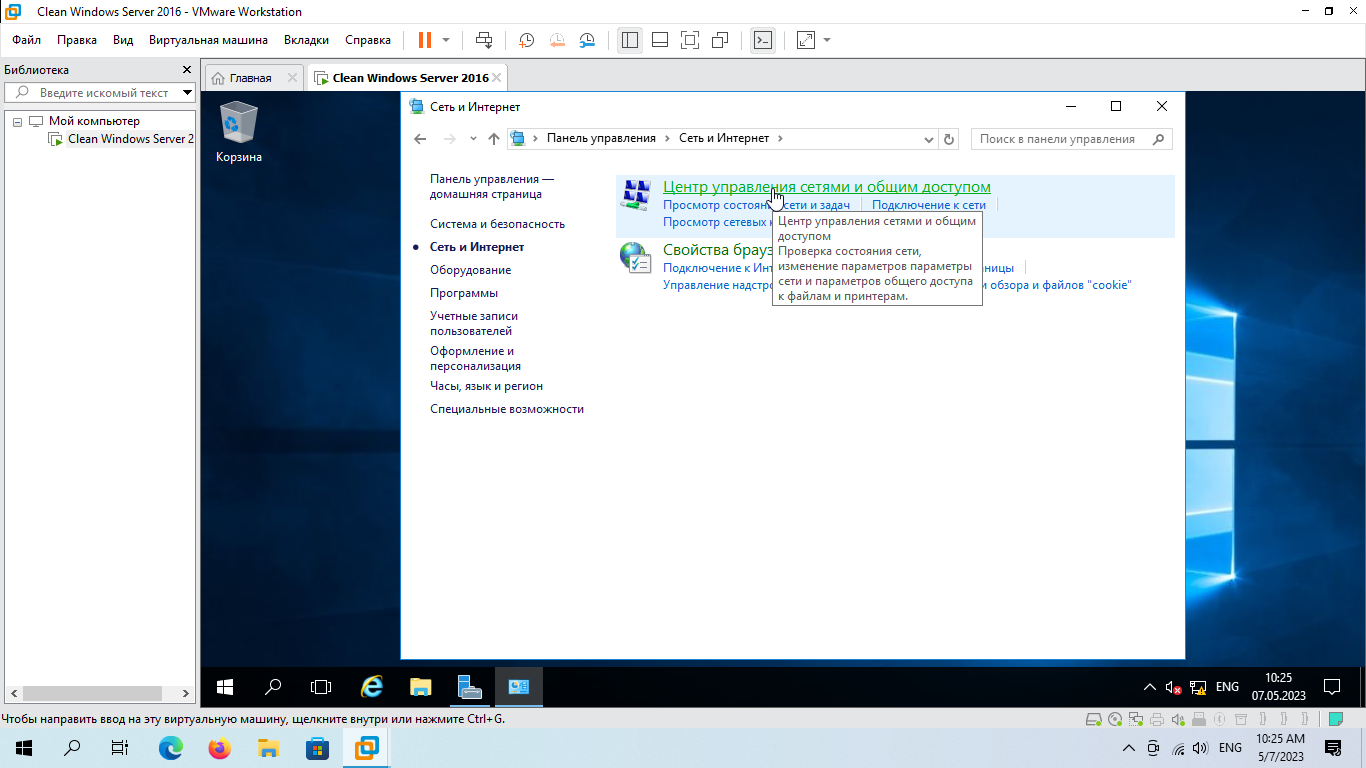
\includegraphics[width=0.85\textwidth]{9_0016}
    \caption{Открываем центр управления сетями и общим доступом}
    \label{img:0016}
  \end{figure}

  \begin{figure}[H]
    \centering
    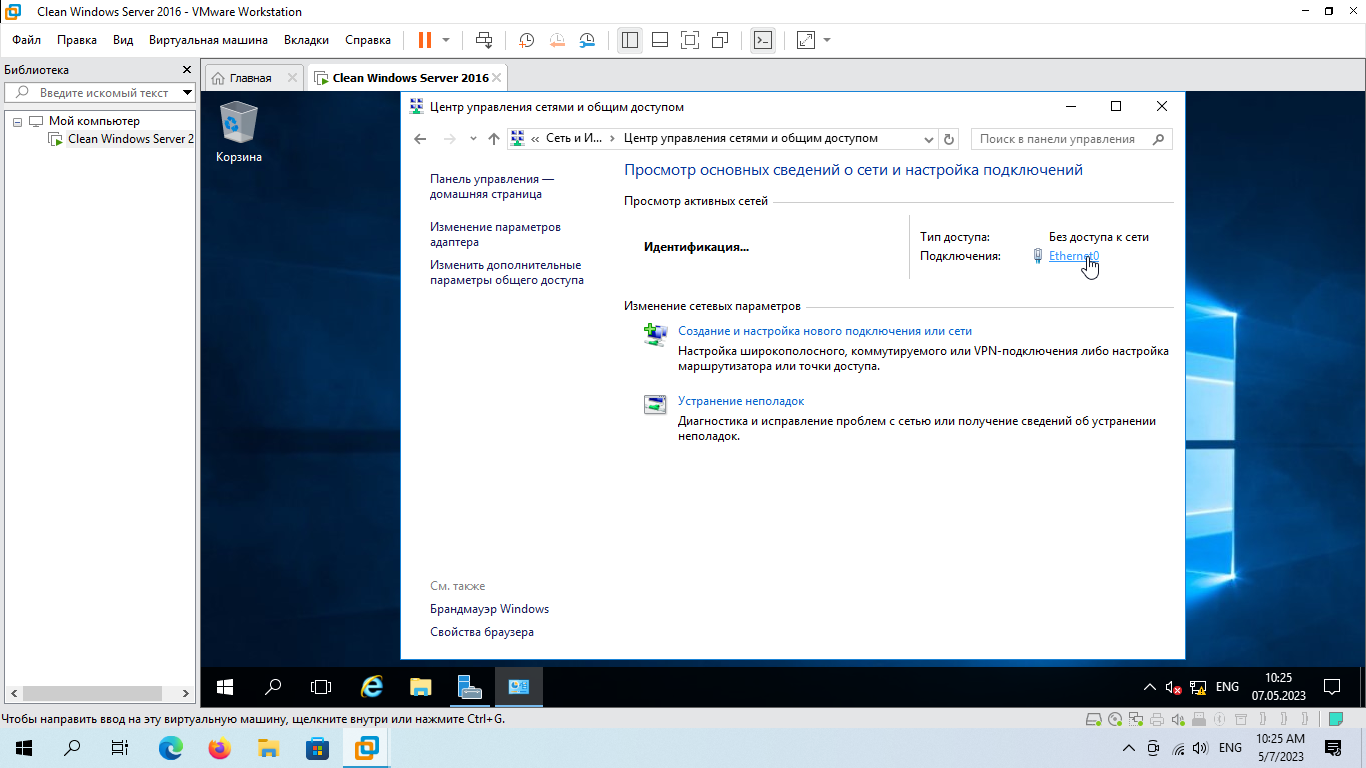
\includegraphics[width=0.85\textwidth]{9_0017}
    \caption{Выбираем необходимый сетевой интерфейс}
    \label{img:0017}
  \end{figure}

  \begin{figure}[H]
    \centering
    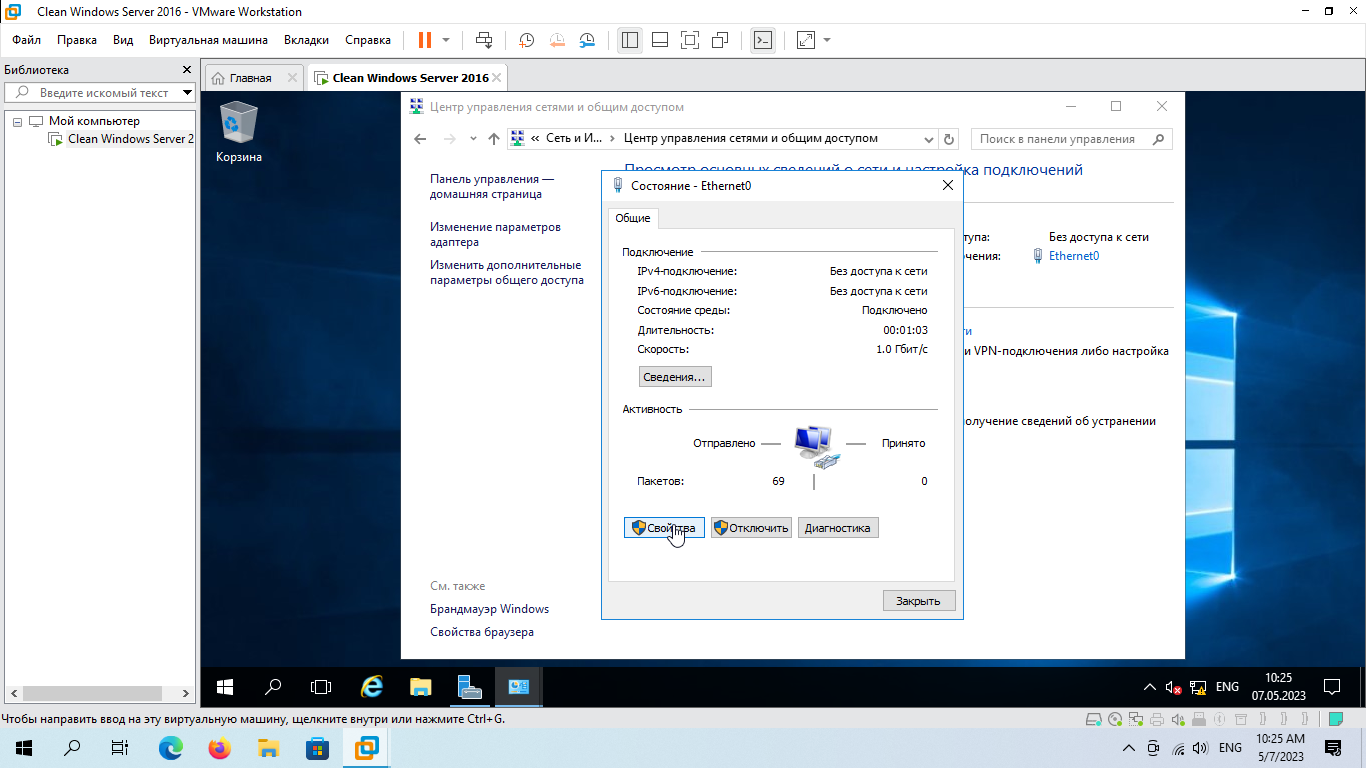
\includegraphics[width=0.85\textwidth]{9_0018}
    \caption{Открываем его свойства}
    \label{img:0018}
  \end{figure}

  \begin{figure}[H]
    \centering
    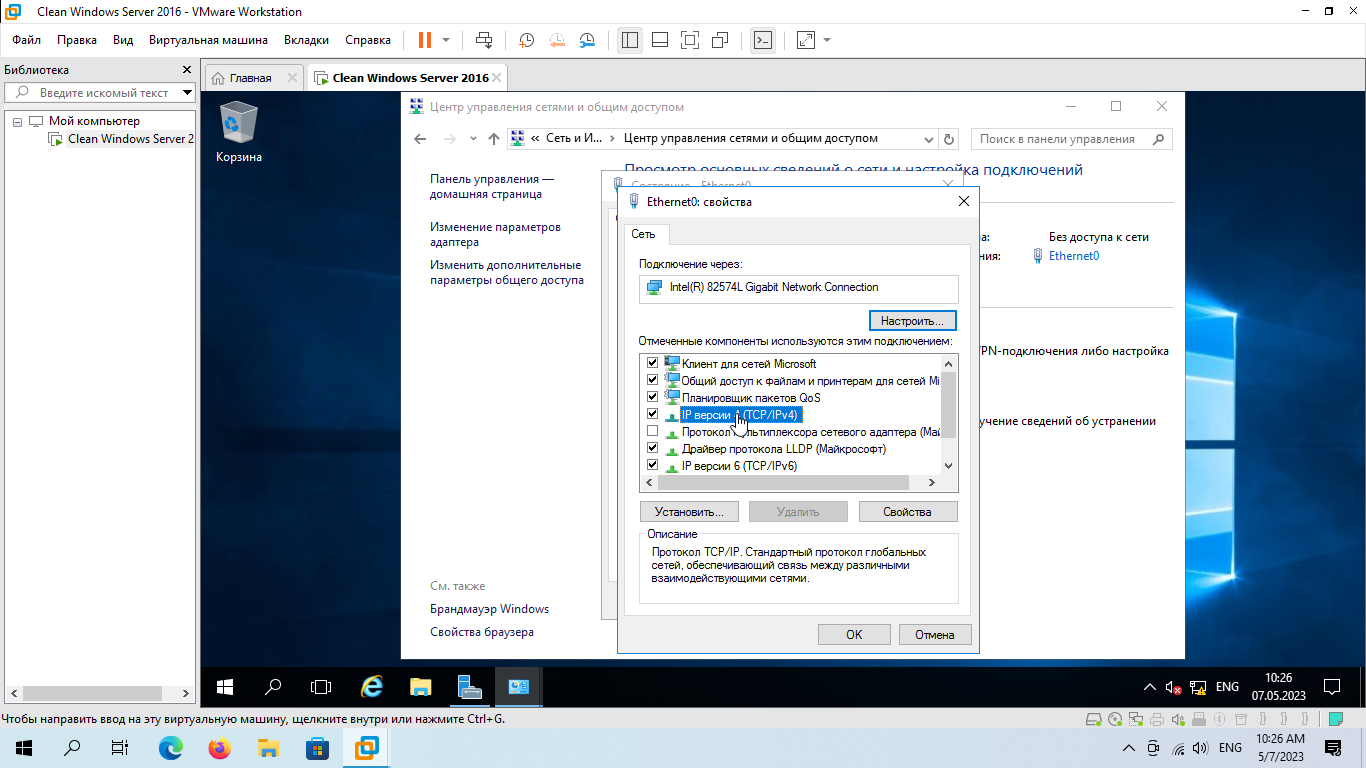
\includegraphics[width=0.85\textwidth]{9_0019}
    \caption{Переходим к настройке IPv4}
    \label{img:0019}
  \end{figure}

  \begin{figure}[H]
    \centering
    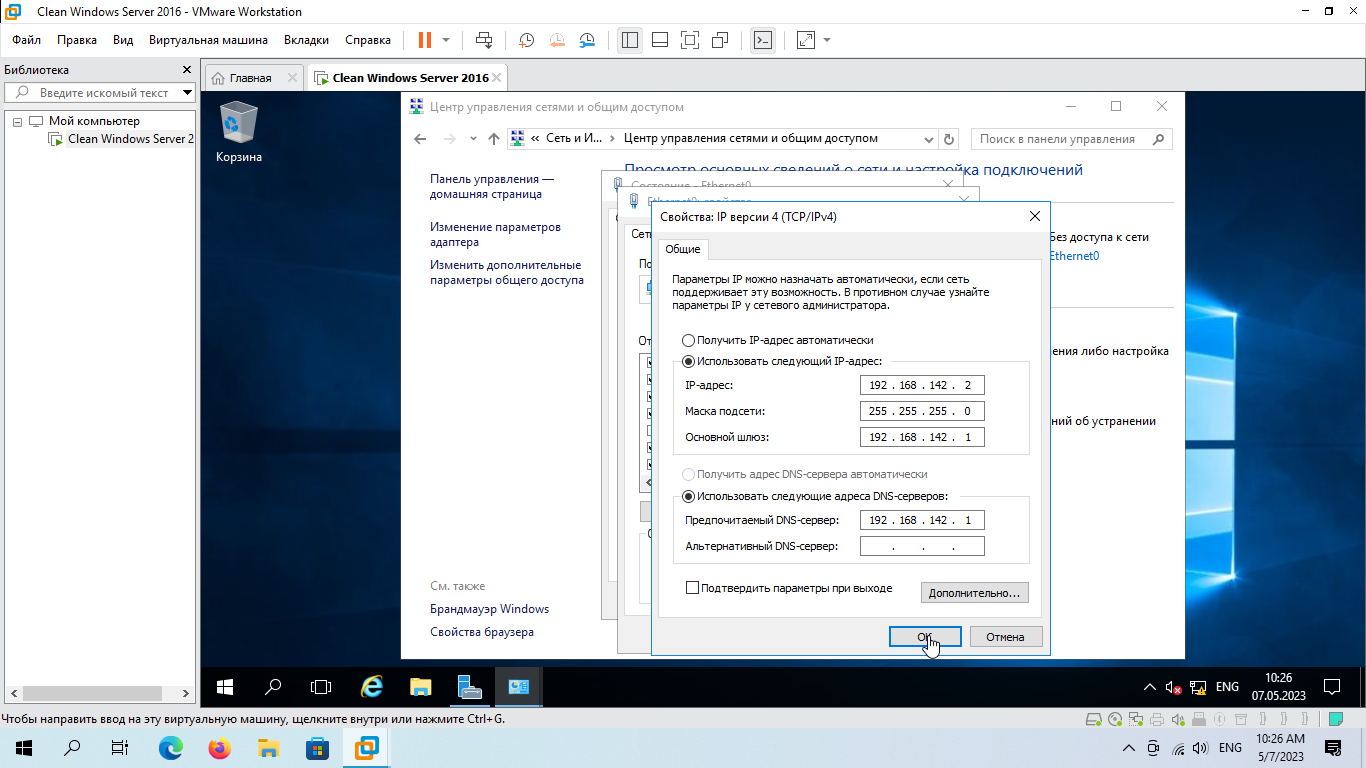
\includegraphics[width=0.85\textwidth]{9_0020}
    \caption{Указываем параметры сети и назначаем IP адрес}
    \label{img:0020}
  \end{figure}

  Параметры сети совпадают с теми, которые были указаны на этапе ее создания,
  в качестве адреса машины опять таки был выбран первый свободный в этой сети -
  192.168.142.2. Адреса шлюза и \textit{DNS} сервера совпадают (пока что).

  \begin{figure}[H]
    \centering
    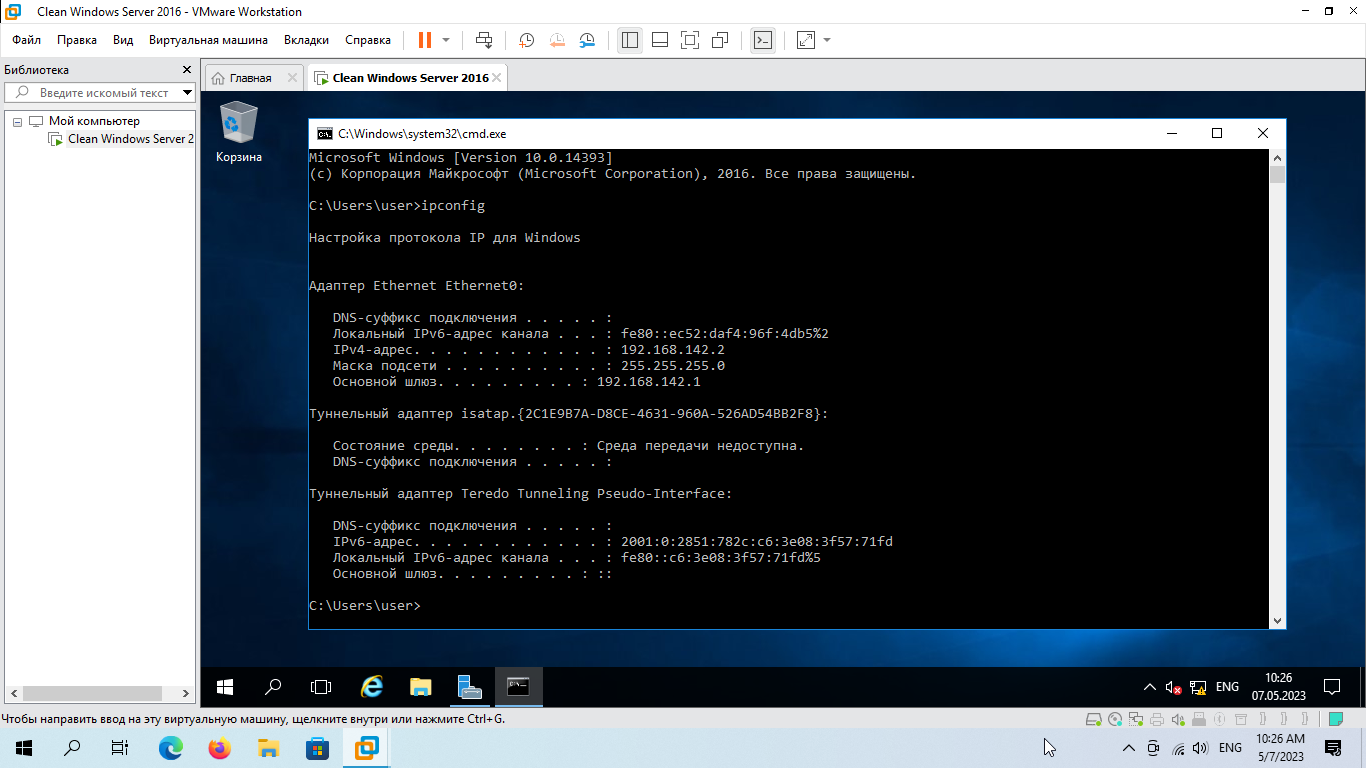
\includegraphics[width=0.85\textwidth]{9_0021}
    \caption{Проверим, что параметры применились при помощи \textit{ipconfig}}
    \label{img:0021}
  \end{figure}

  также необходимо удостовериться, что работает доступ в сеть, машина может достучаться
  до шлюза и выполнить \textit{DNS} запрос:

  \begin{figure}[H]
    \centering
    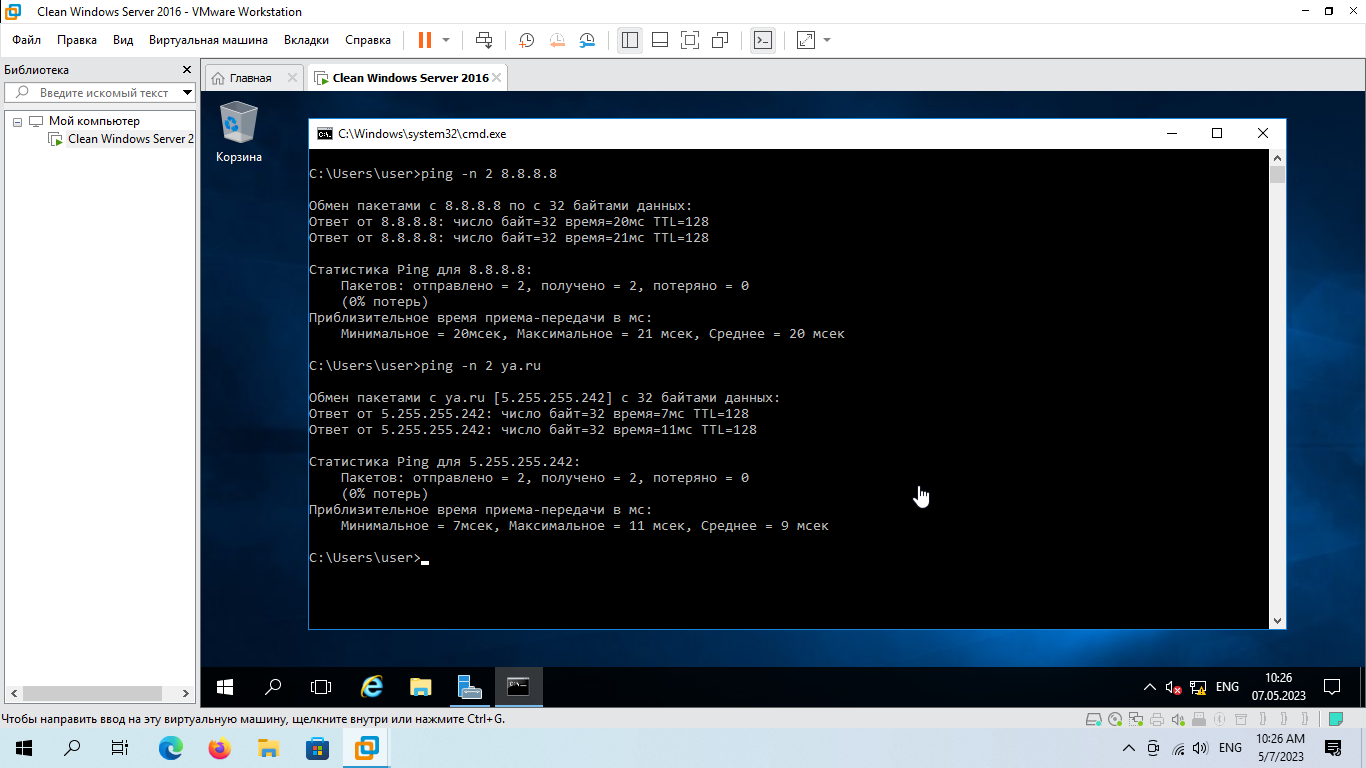
\includegraphics[width=0.85\textwidth]{9_0022}
    \caption{ping google dns and ya.ru}
    \label{img:0022}
  \end{figure}

  \begin{figure}[H]
    \centering
    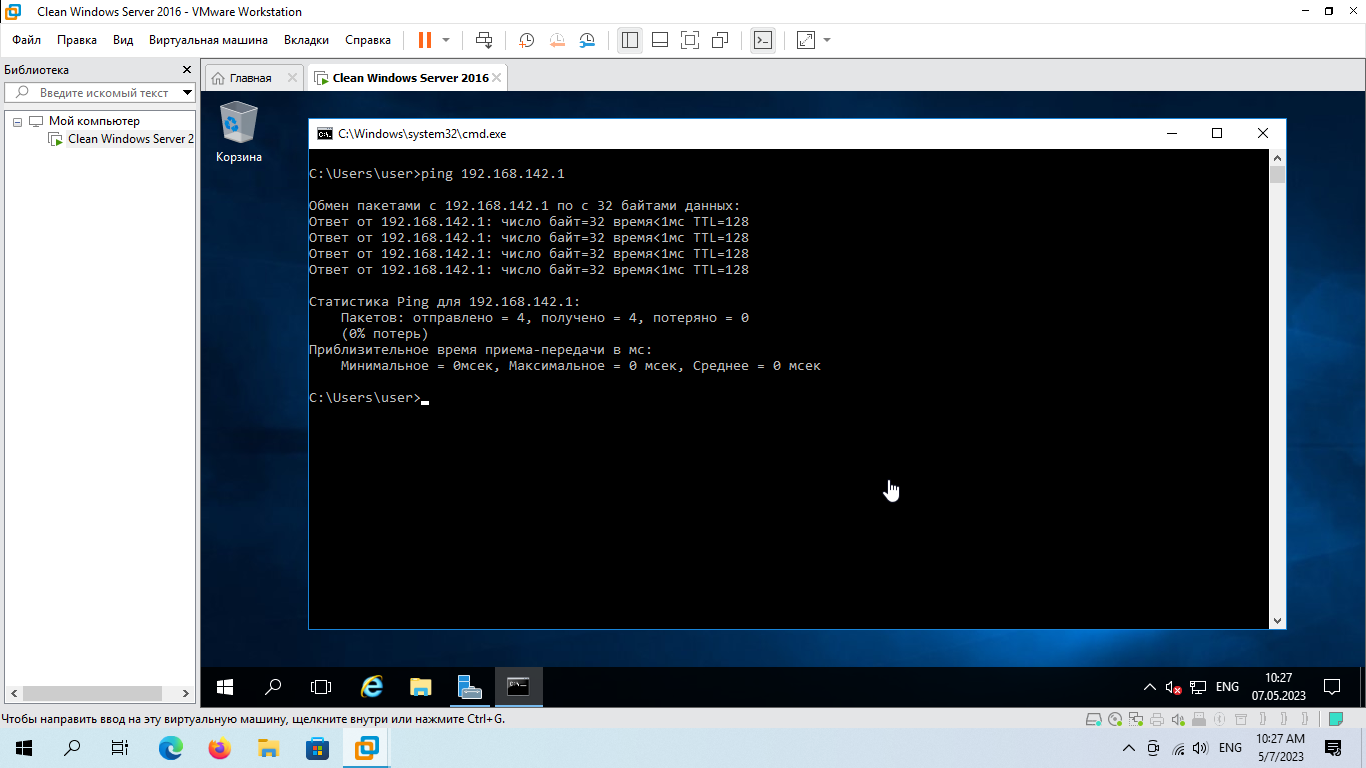
\includegraphics[width=0.85\textwidth]{9_0023}
    \caption{ping gateway}
    \label{img:0023}
  \end{figure}

  Сеть настроена и работает.

  \subsubsection{Задание пароля Администратора}

  \begin{figure}[H]
    \centering
    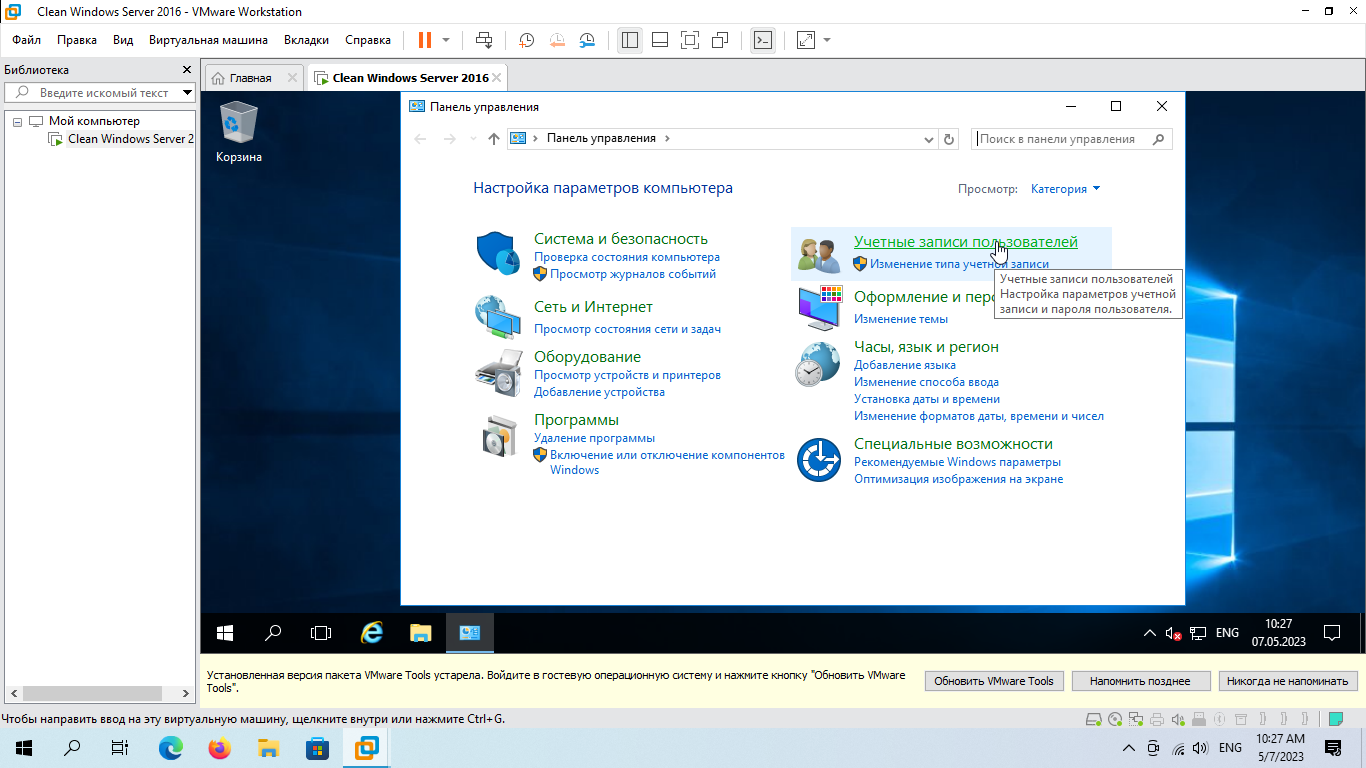
\includegraphics[width=0.85\textwidth]{9_0024}
    \caption{В панели управления открываем "Учетные записи пользователей"}
    \label{img:0024}
  \end{figure}

  \begin{figure}[H]
    \centering
    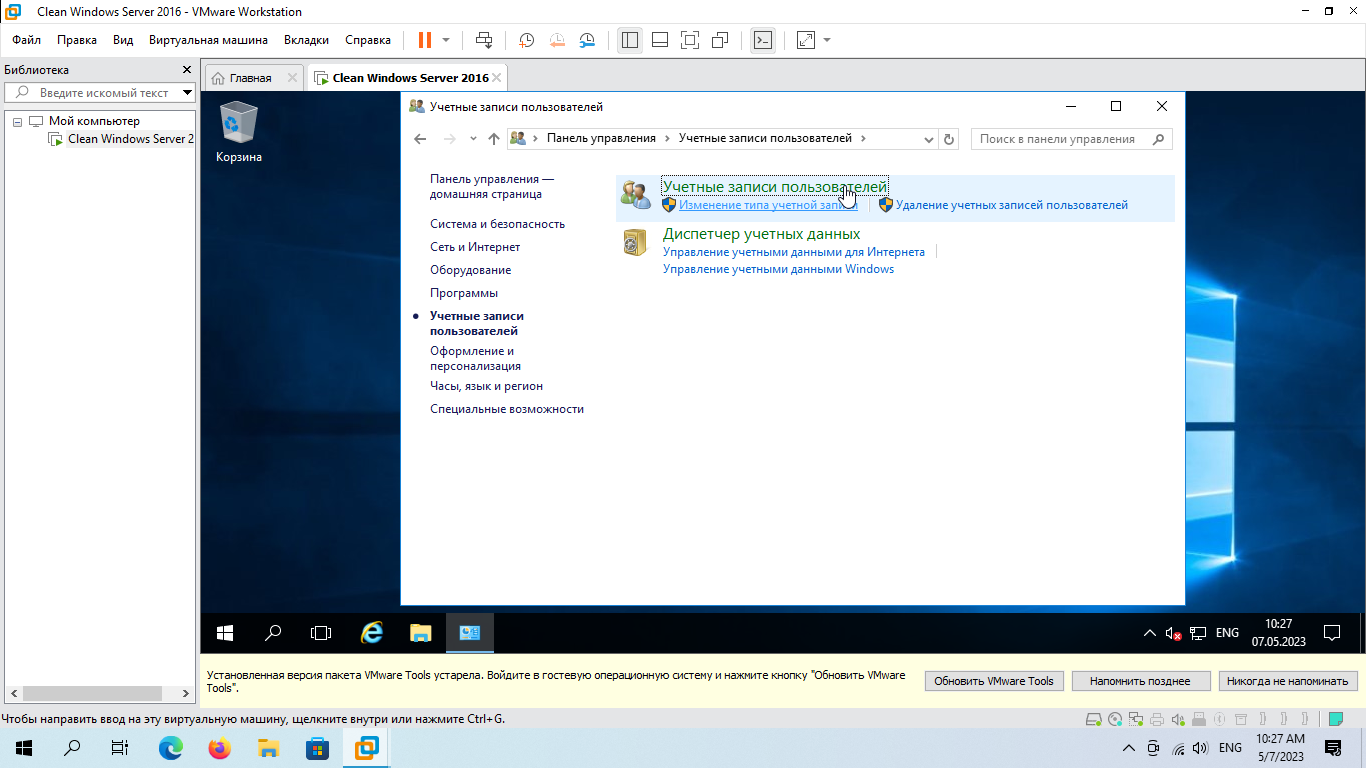
\includegraphics[width=0.85\textwidth]{9_0025}
    \caption{Снова туда же}
    \label{img:0025}
  \end{figure}

  \begin{figure}[H]
    \centering
    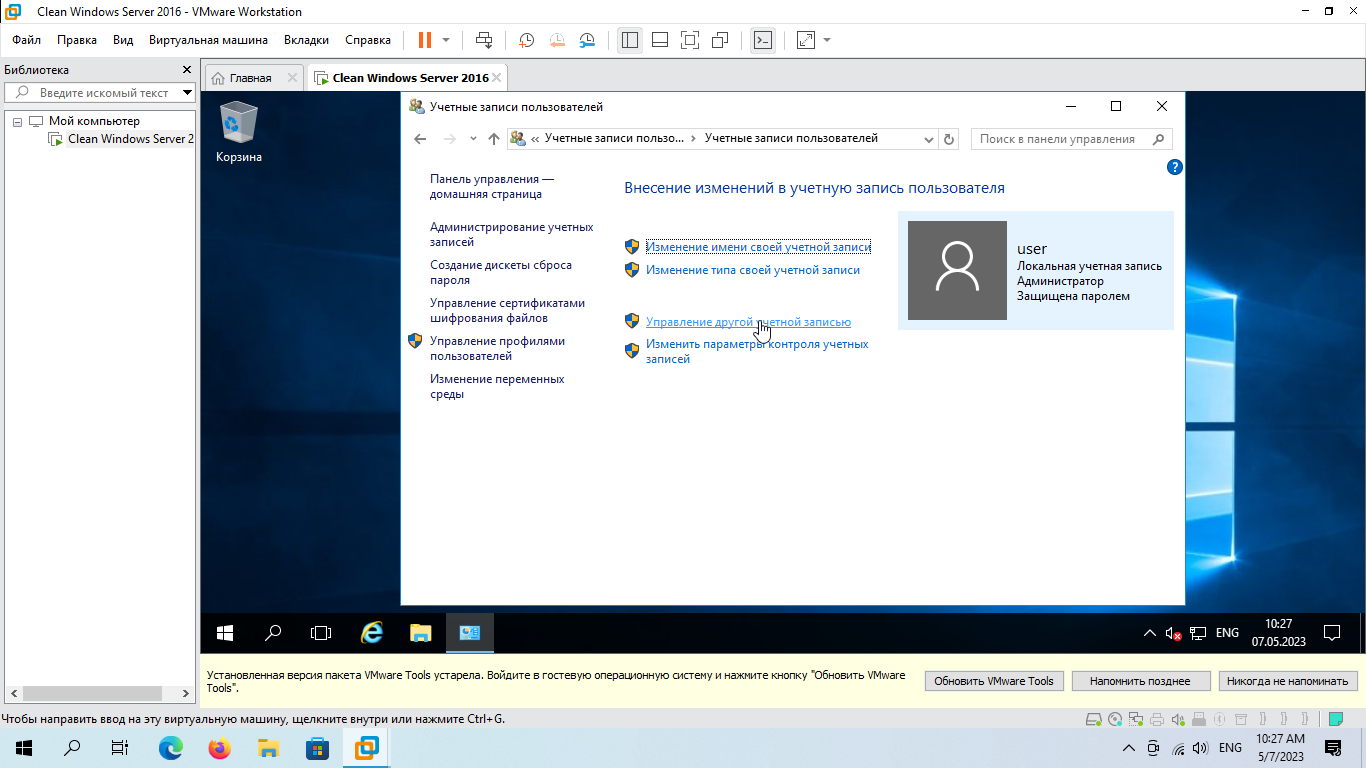
\includegraphics[width=0.85\textwidth]{9_0026}
    \caption{Управления другой учетной записью}
    \label{img:0026}
  \end{figure}

  \begin{figure}[H]
    \centering
    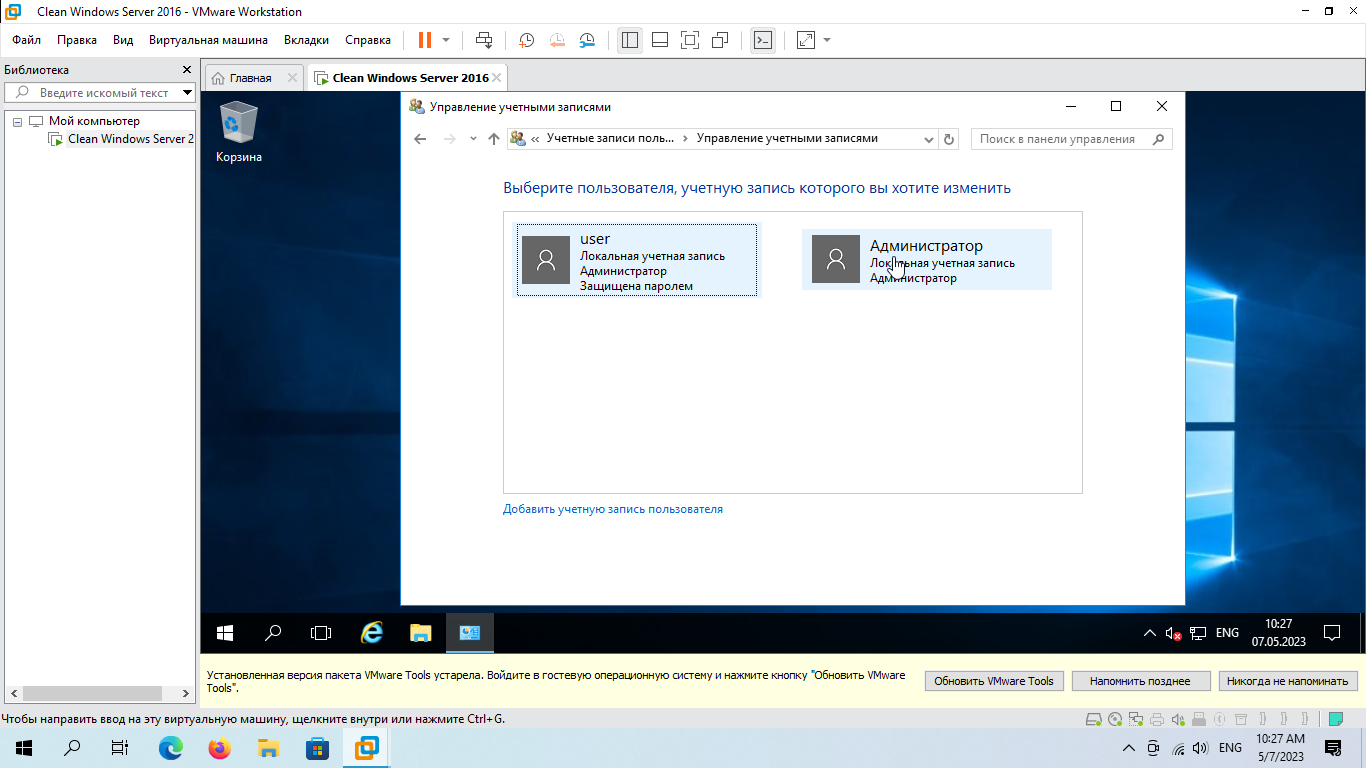
\includegraphics[width=0.85\textwidth]{9_0027}
    \caption{Выбираем Администратора}
    \label{img:0027}
  \end{figure}

  \begin{figure}[H]
    \centering
    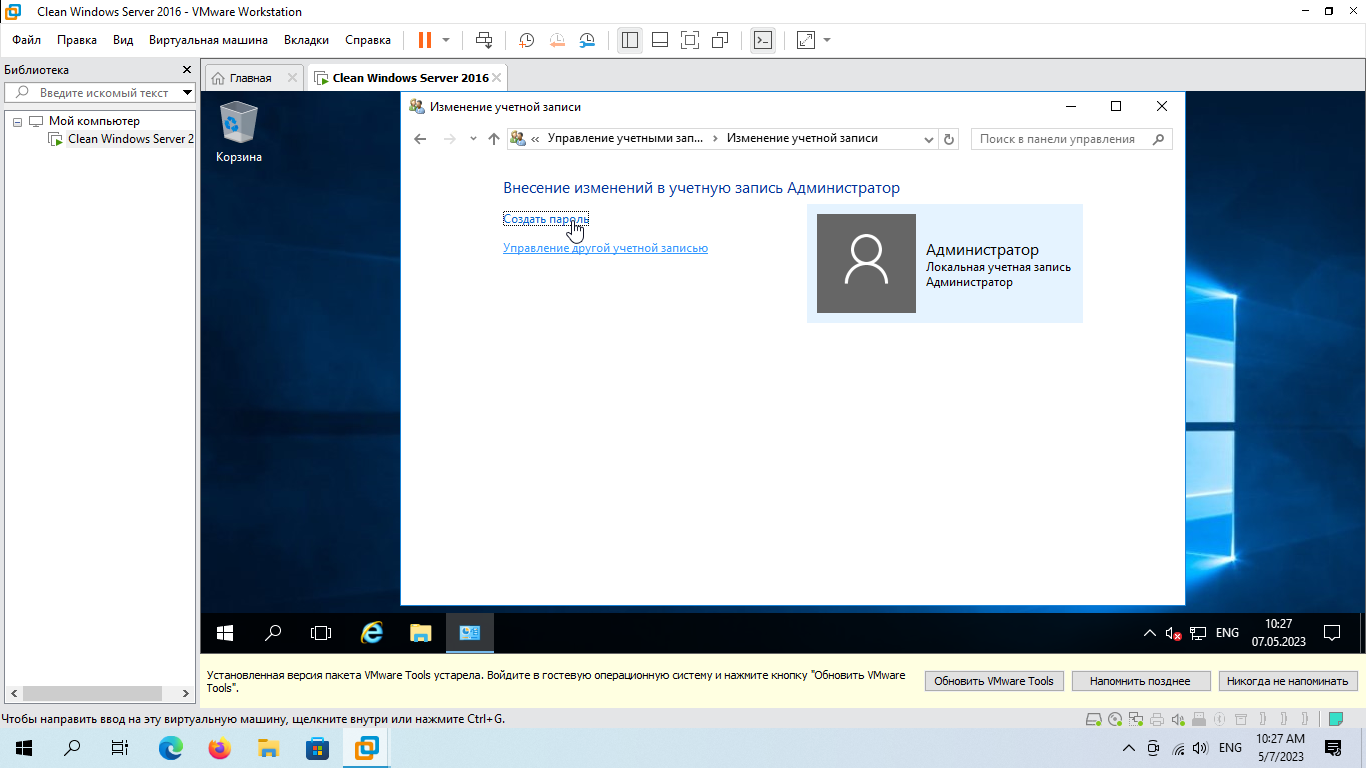
\includegraphics[width=0.85\textwidth]{9_0028}
    \caption{Начинаем процесс смены пароля}
    \label{img:0028}
  \end{figure}

  \begin{figure}[H]
    \centering
    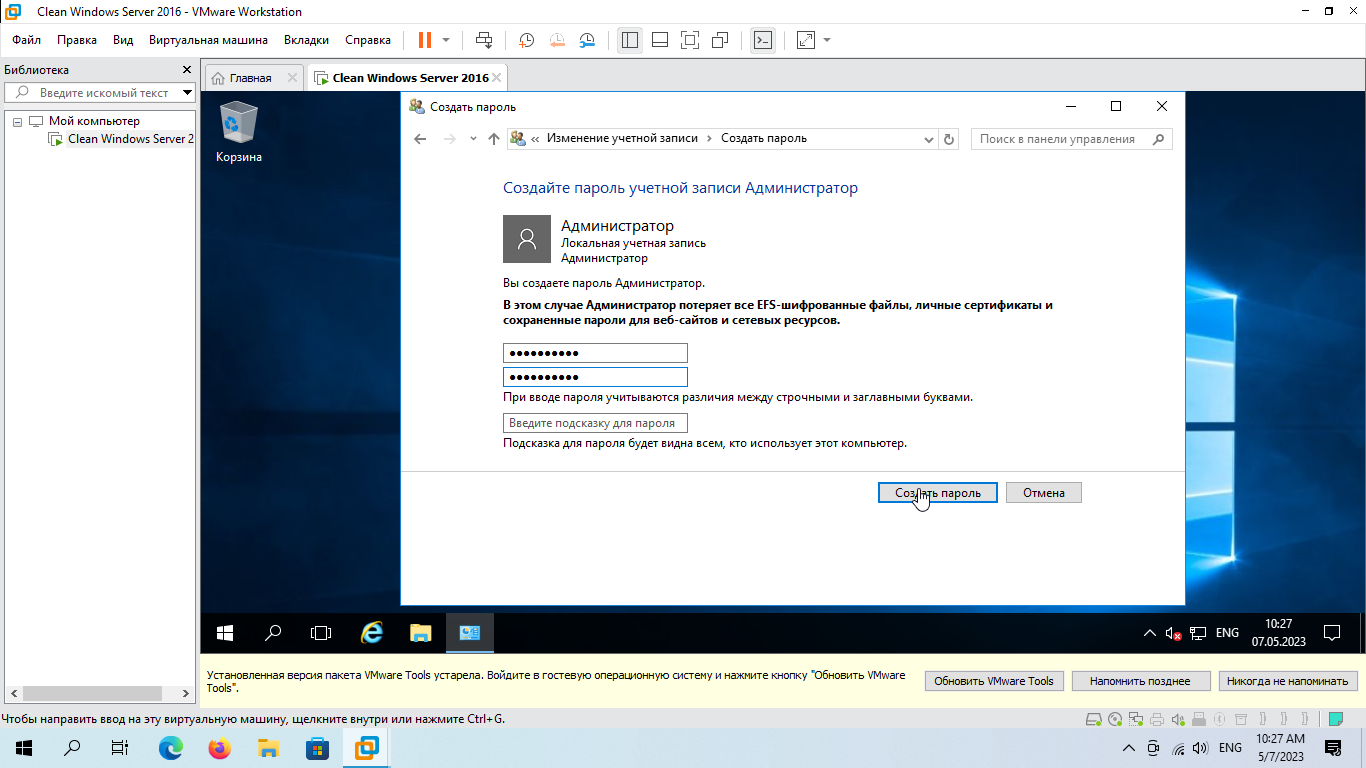
\includegraphics[width=0.85\textwidth]{9_0030}
    \caption{Указываем новый пароль}
    \label{img:0030}
  \end{figure}

  \subsubsection{Установка необходимых компонентов}

  \begin{figure}[H]
    \centering
    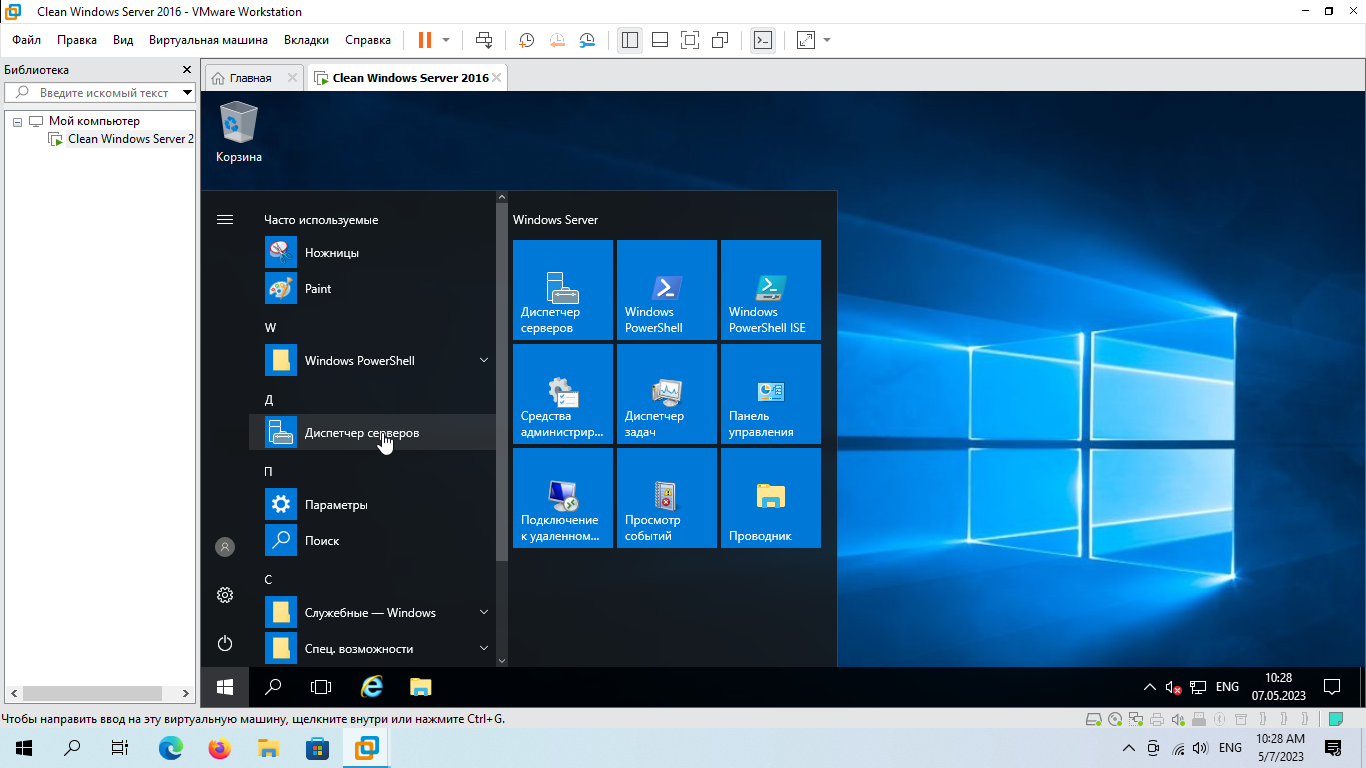
\includegraphics[width=0.85\textwidth]{9_0031}
    \caption{Открываем диспетчер серверов}
    \label{img:0031}
  \end{figure}

  \begin{figure}[H]
    \centering
    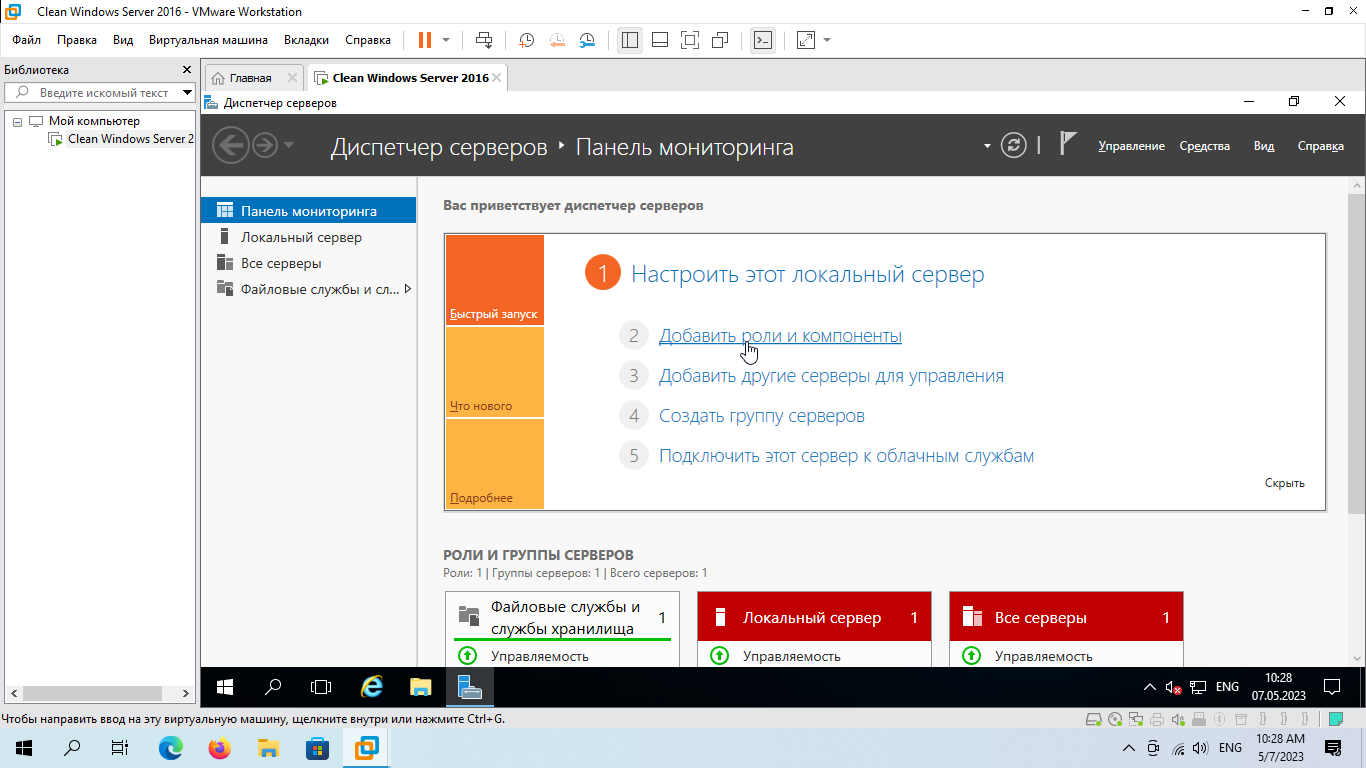
\includegraphics[width=0.85\textwidth]{9_0032}
    \caption{Начинаем добавление ролей и компонентов}
    \label{img:0032}
  \end{figure}

  \begin{figure}[H]
    \centering
    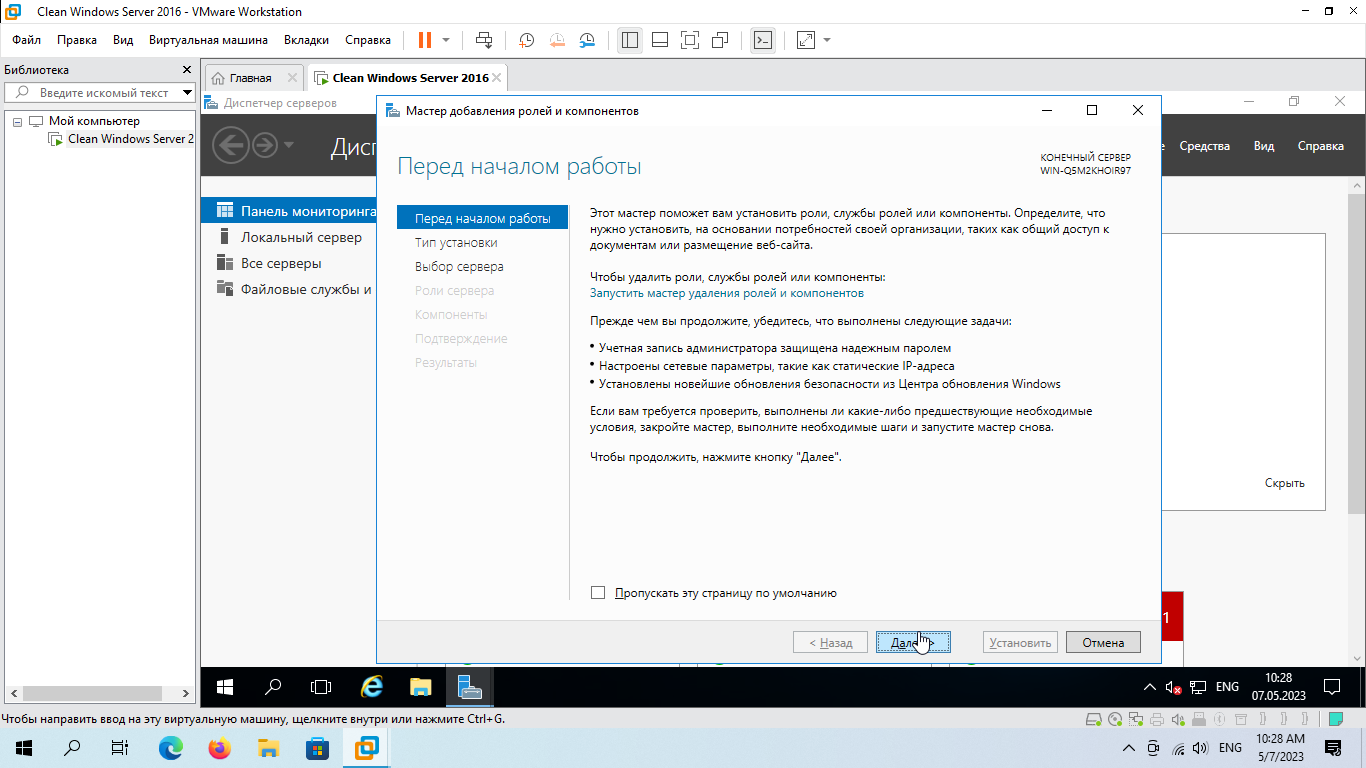
\includegraphics[width=0.85\textwidth]{9_0033}
    \caption{Далее}
    \label{img:0033}
  \end{figure}

  \begin{figure}[H]
    \centering
    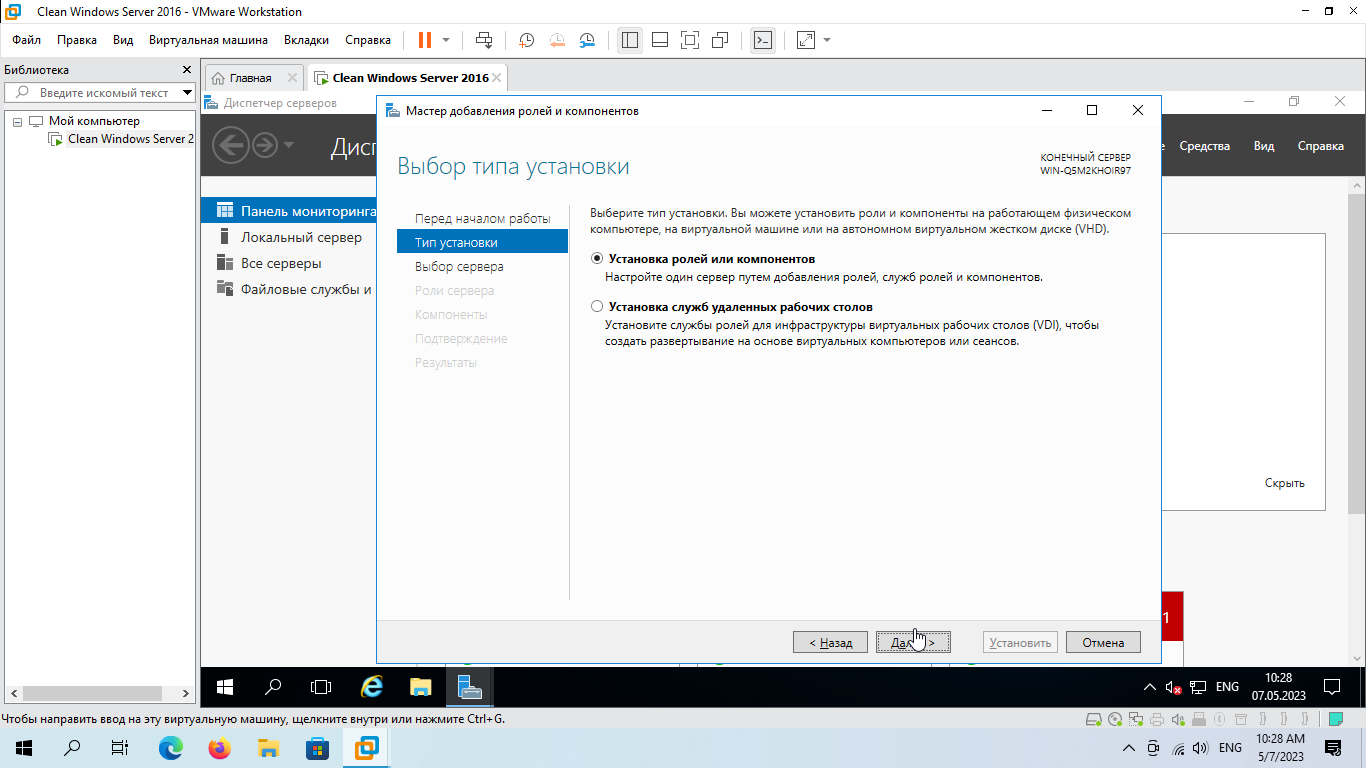
\includegraphics[width=0.85\textwidth]{9_0034}
    \caption{Нам нужны роли: роль \textit{DNS} сервера и \textit{AD DS}}
    \label{img:0034}
  \end{figure}

  \begin{figure}[H]
    \centering
    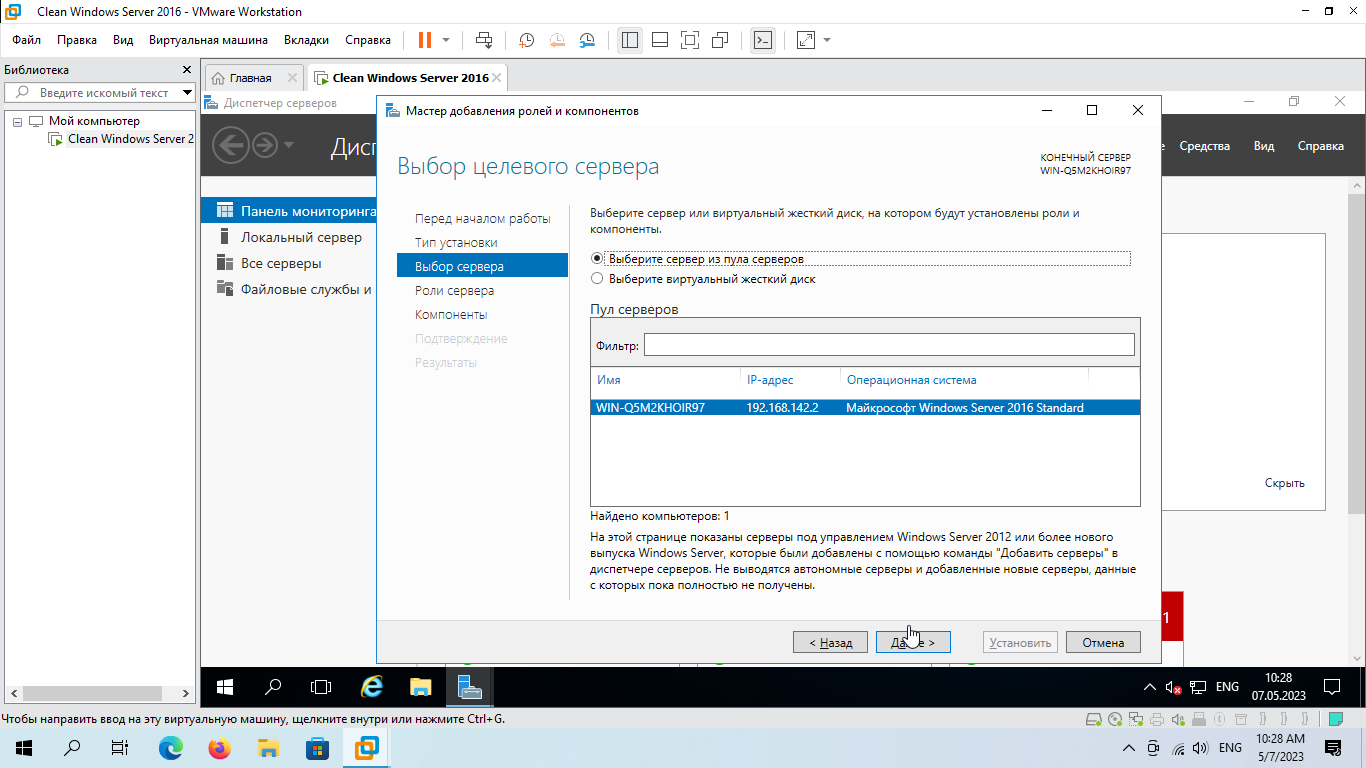
\includegraphics[width=0.85\textwidth]{9_0035}
    \caption{Выполняем установку для текущего компьютера}
    \label{img:0035}
  \end{figure}

  \begin{figure}[H]
    \centering
    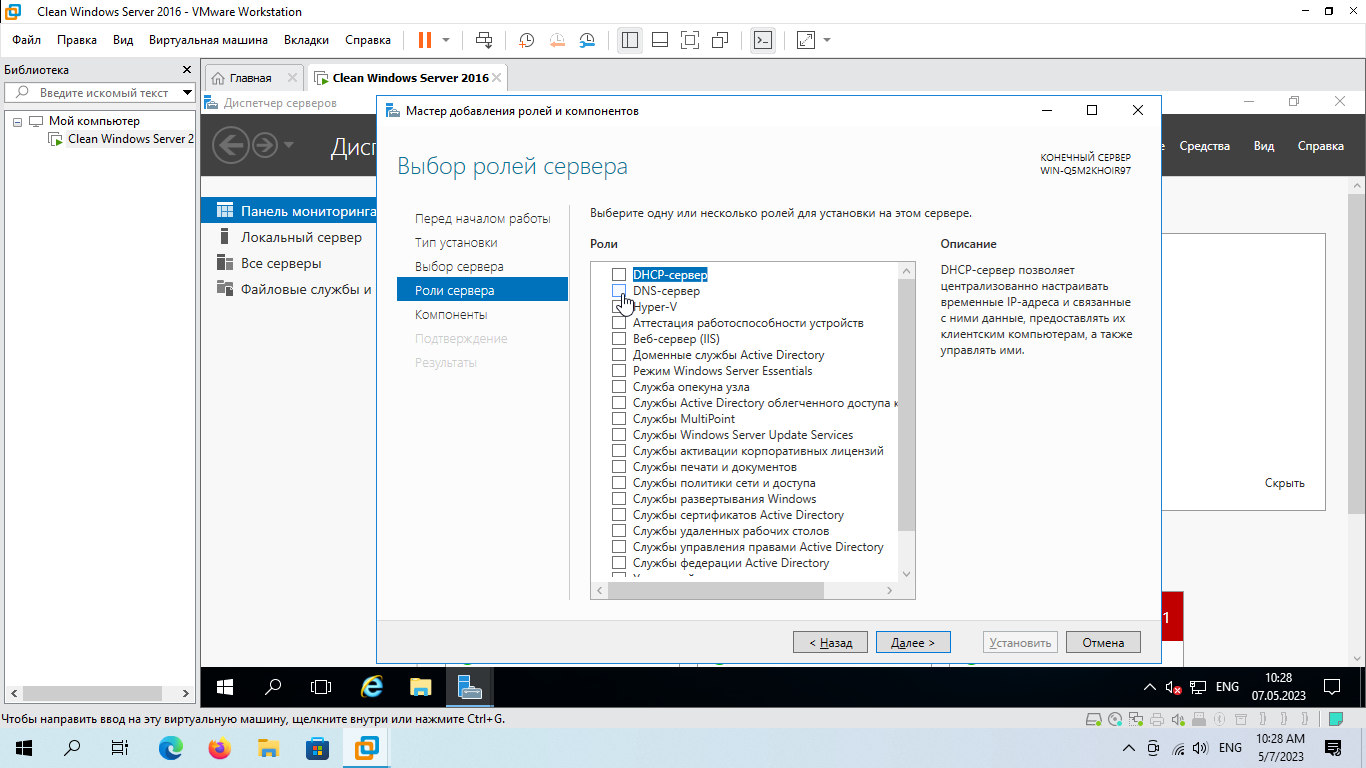
\includegraphics[width=0.85\textwidth]{9_0036}
    \caption{Добавляем роль \textit{DNS} сервера}
    \label{img:0036}
  \end{figure}

  \begin{figure}[H]
    \centering
    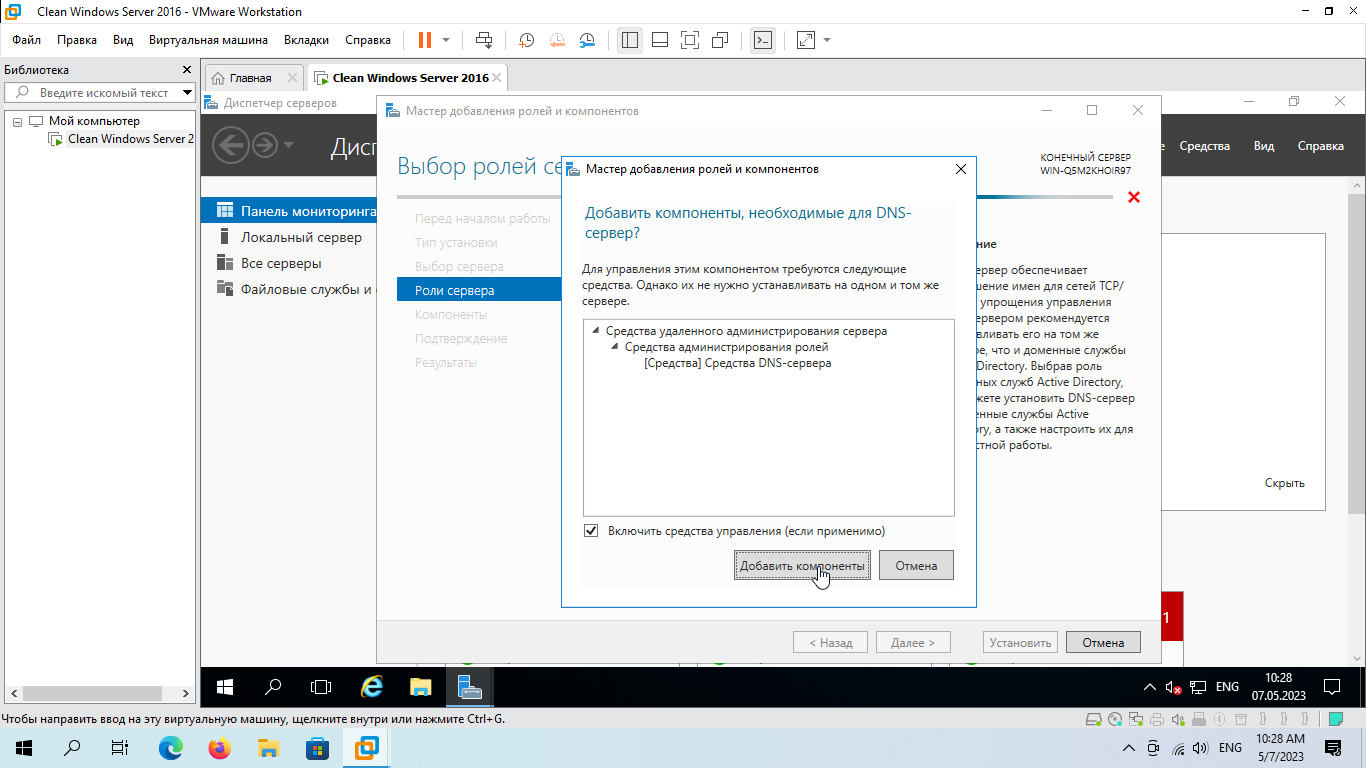
\includegraphics[width=0.85\textwidth]{9_0037}
    \caption{И необходимые для нее компоненты}
    \label{img:0037}
  \end{figure}

  \begin{figure}[H]
    \centering
    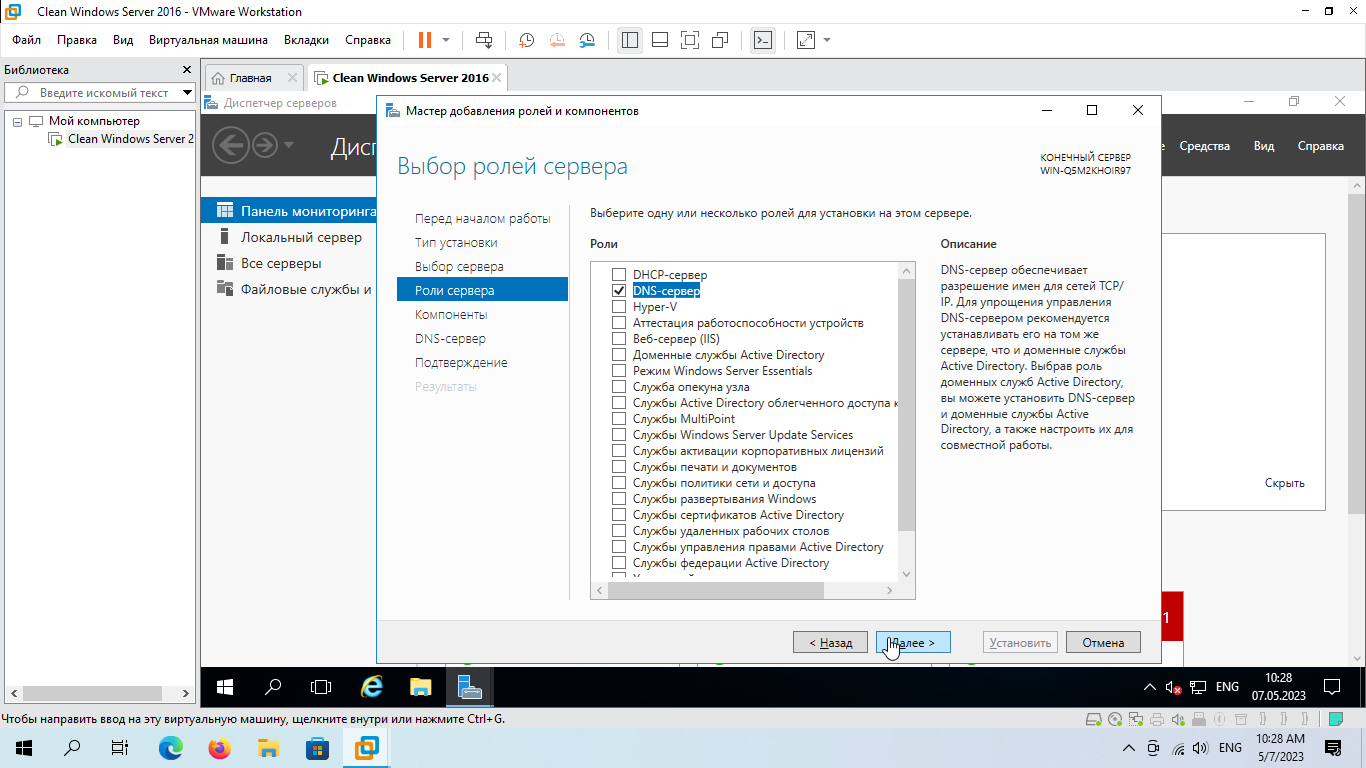
\includegraphics[width=0.85\textwidth]{9_0038}
    \caption{Далее}
    \label{img:0038}
  \end{figure}

  \begin{figure}[H]
    \centering
    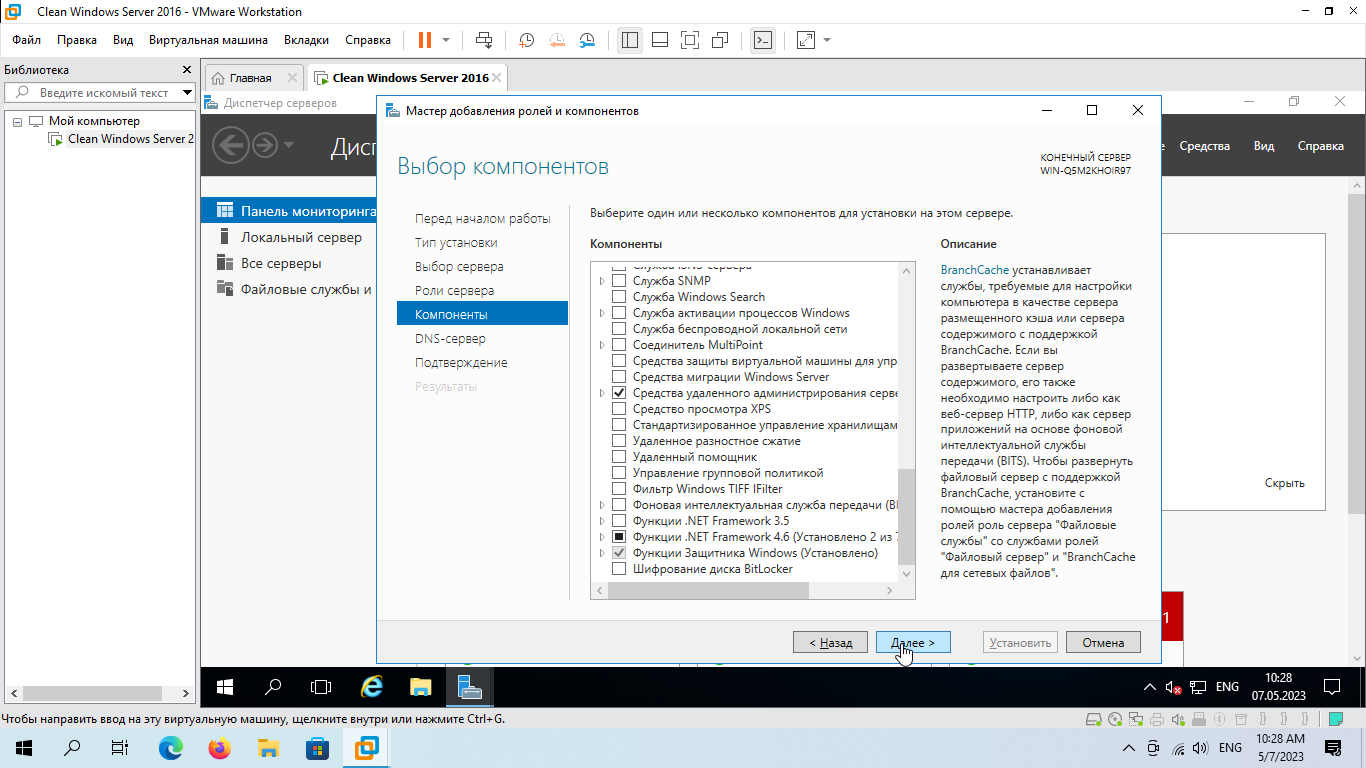
\includegraphics[width=0.85\textwidth]{9_0040}
    \caption{Далее}
    \label{img:0040}
  \end{figure}

  \begin{figure}[H]
    \centering
    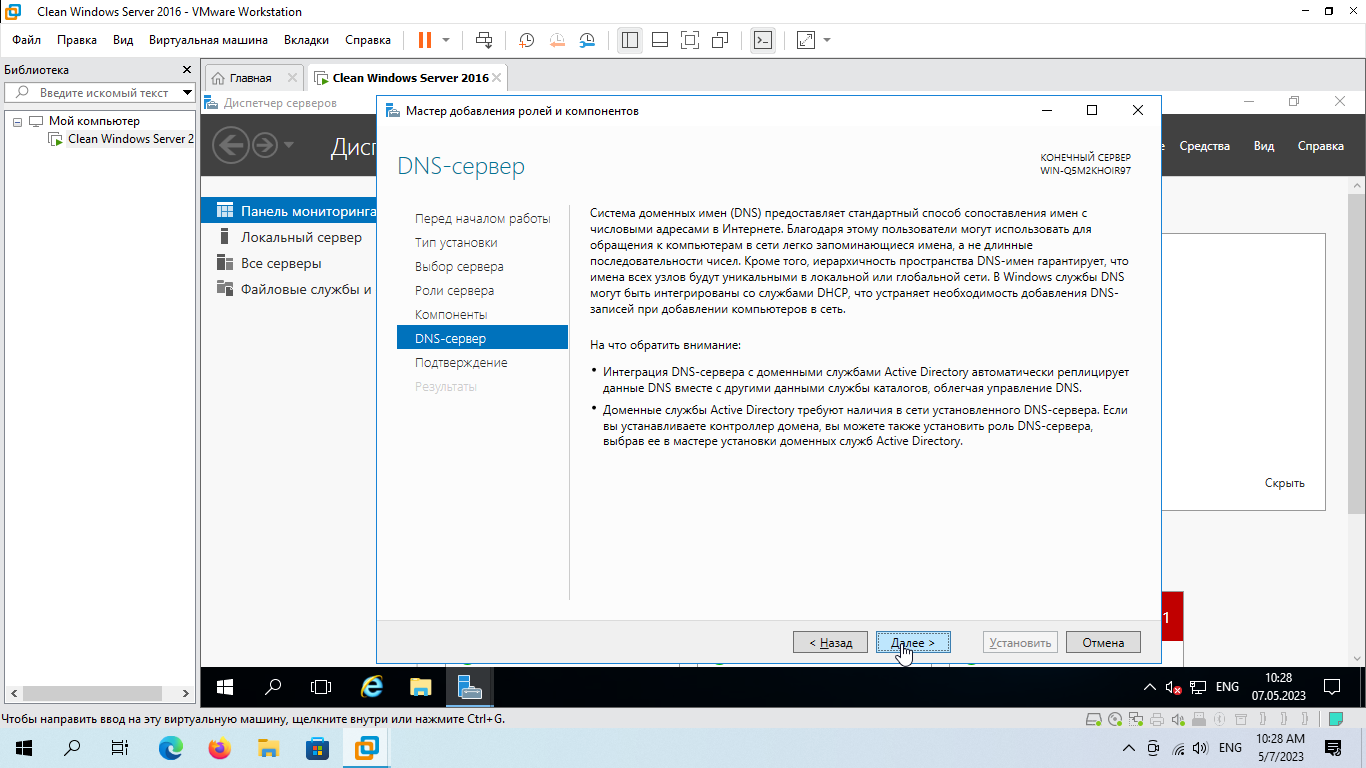
\includegraphics[width=0.85\textwidth]{9_0041}
    \caption{Далее}
    \label{img:0041}
  \end{figure}

  \begin{figure}[H]
    \centering
    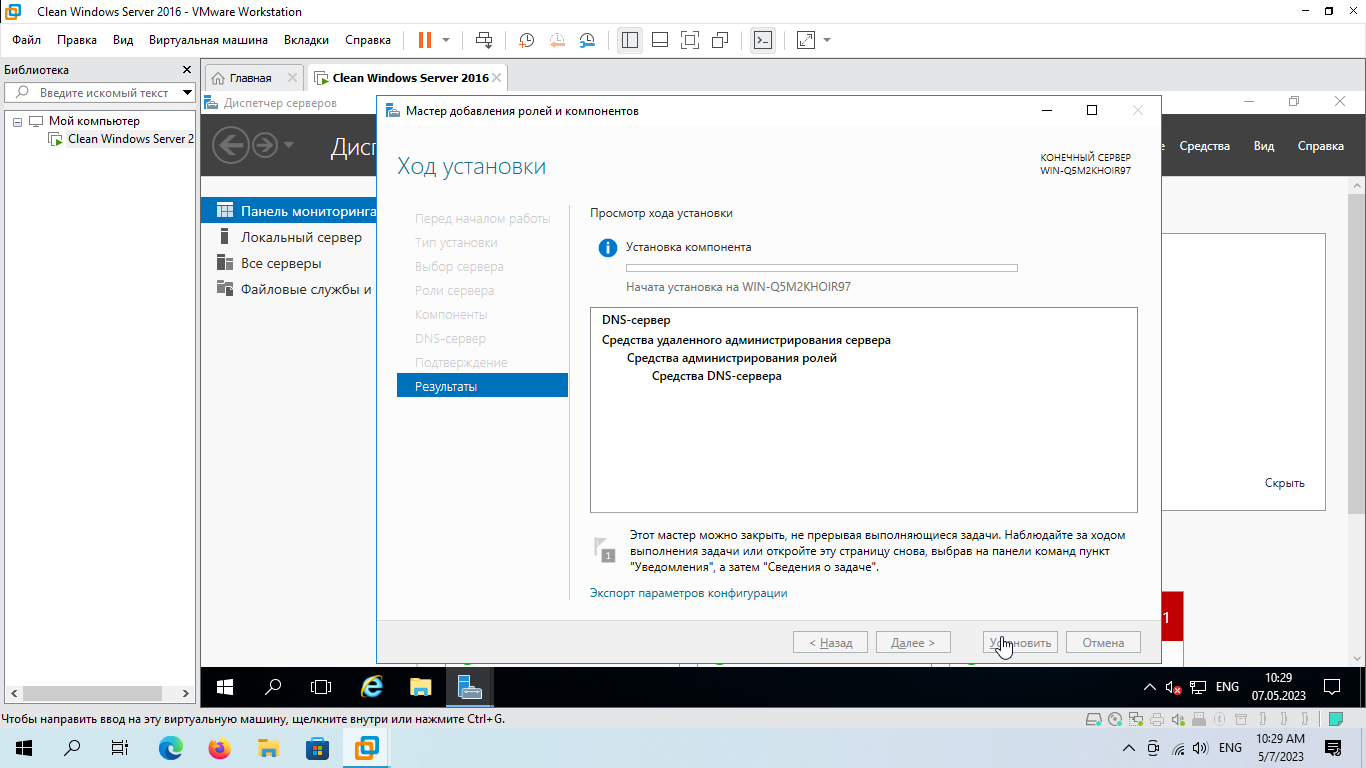
\includegraphics[width=0.85\textwidth]{9_0042}
    \caption{Выполняется установка \textit{DNS} роли и необходимых компонентов}
    \label{img:0042}
  \end{figure}
  
  \begin{figure}[H]
    \centering
    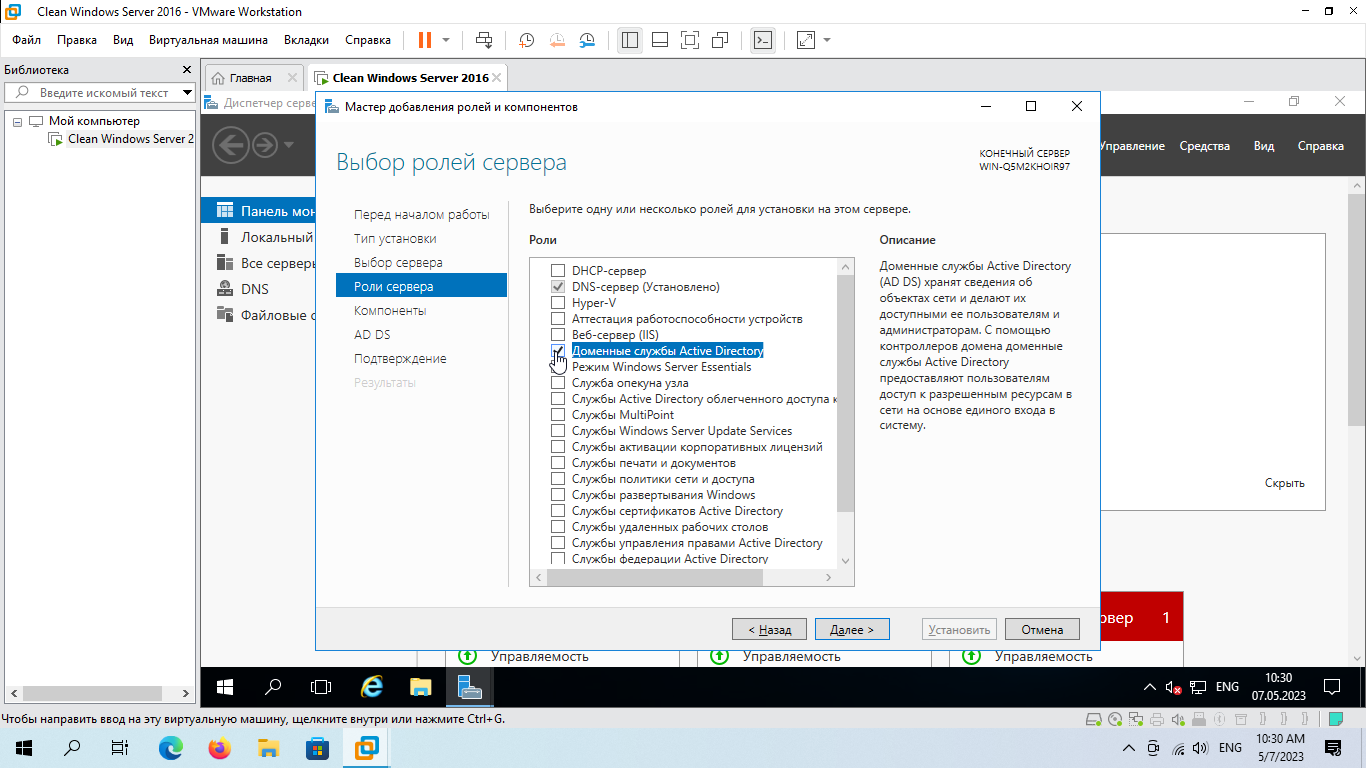
\includegraphics[width=0.85\textwidth]{9_0047}
    \caption{Аналогично добавляем \textit{AD DS}}
    \label{img:0046}
  \end{figure}

  \begin{figure}[H]
    \centering
    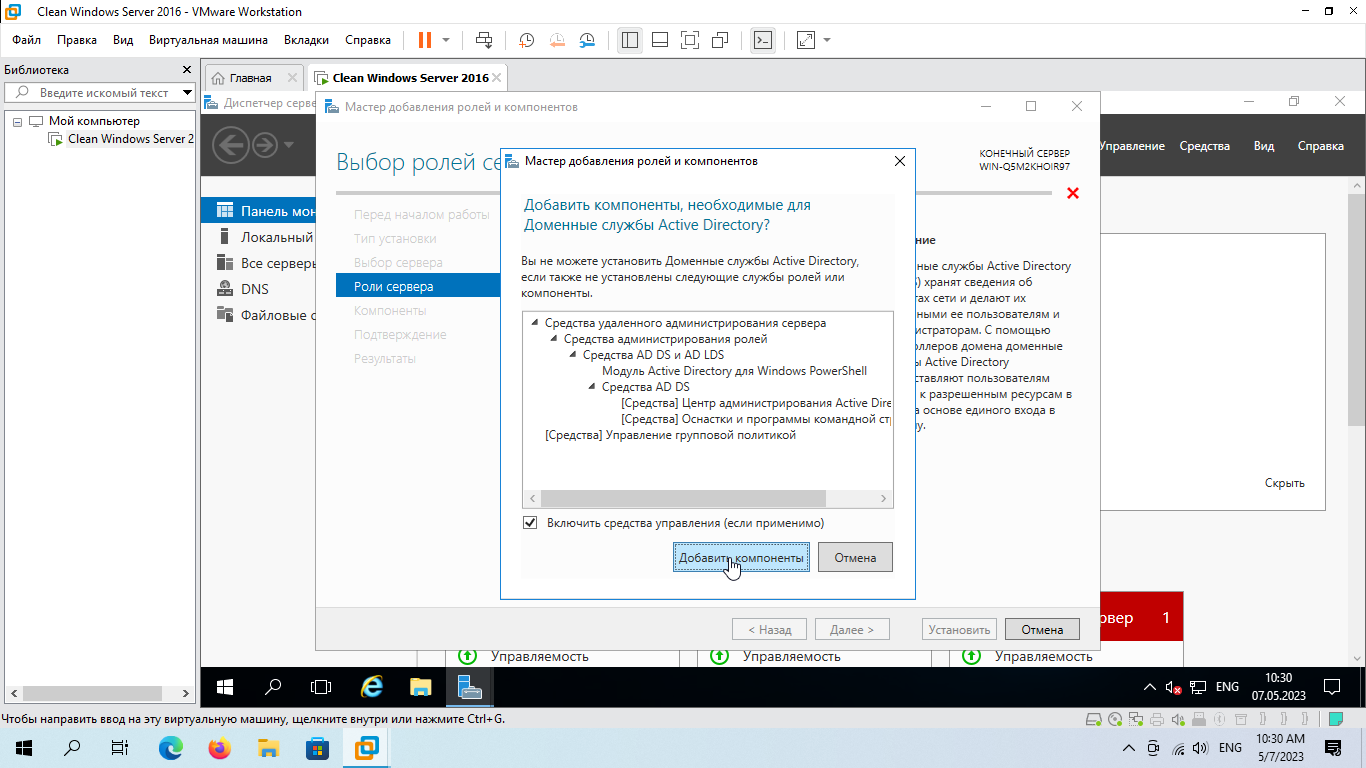
\includegraphics[width=0.85\textwidth]{9_0046}
    \caption{И необходимые для \textit{AD DS} компоненты}
    \label{img:0047}
  \end{figure}

  \begin{figure}[H]
    \centering
    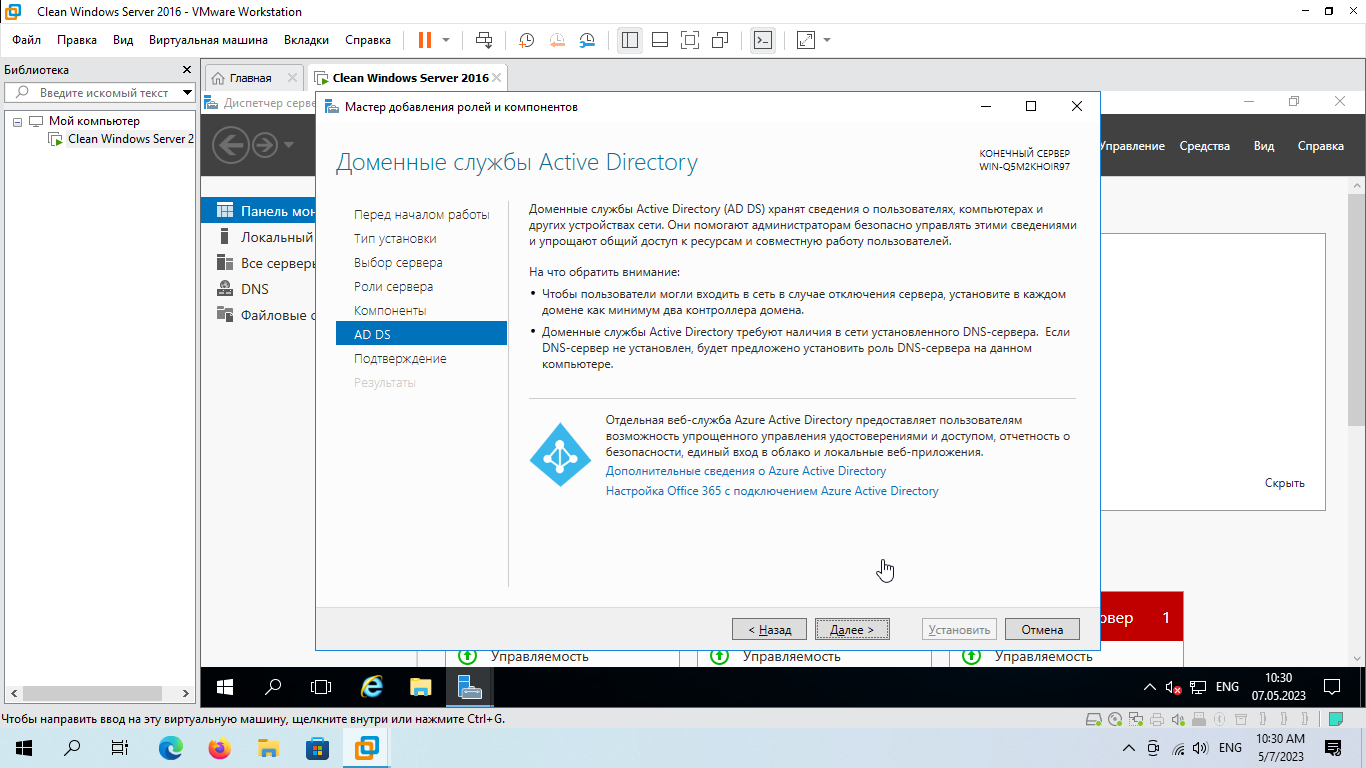
\includegraphics[width=0.85\textwidth]{9_0048}
    \caption{Далее}
    \label{img:0048}
  \end{figure}

  \begin{figure}[H]
    \centering
    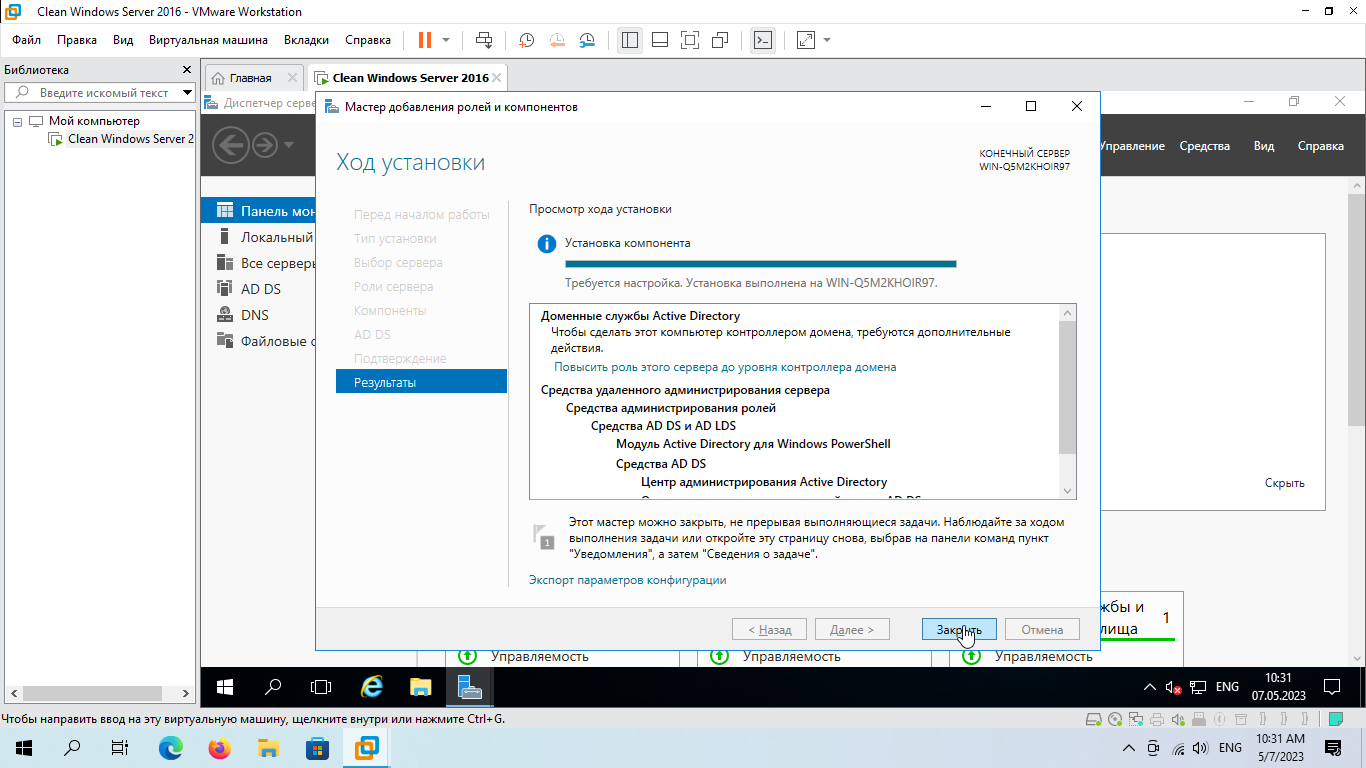
\includegraphics[width=0.85\textwidth]{9_0049}
    \caption{Все роли и компоненты установлены}
    \label{img:0049}
  \end{figure}

  \subsubsection{Настройка домена}

  \begin{figure}[H]
    \centering
    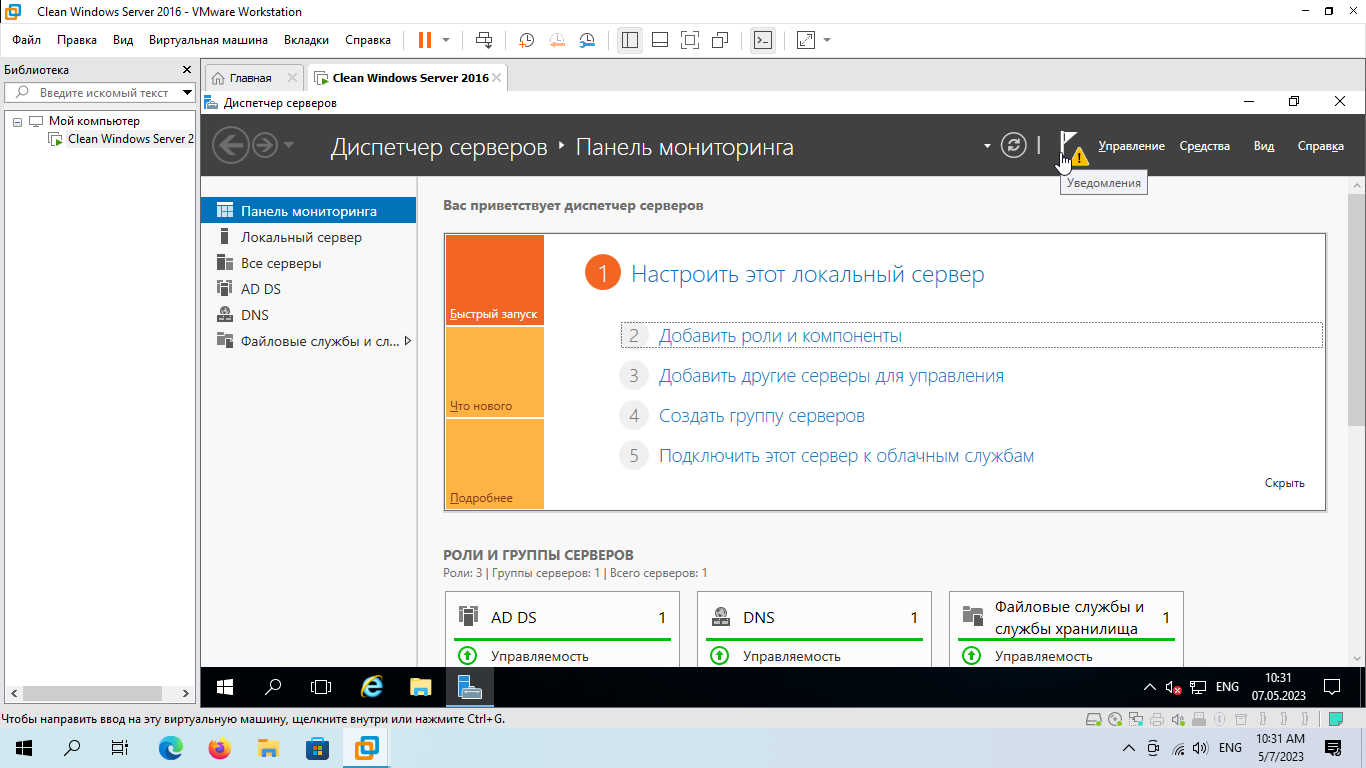
\includegraphics[width=0.85\textwidth]{9_0050}
    \caption{Открываем уведомления}
    \label{img:0050}
  \end{figure}

  \begin{figure}[H]
    \centering
    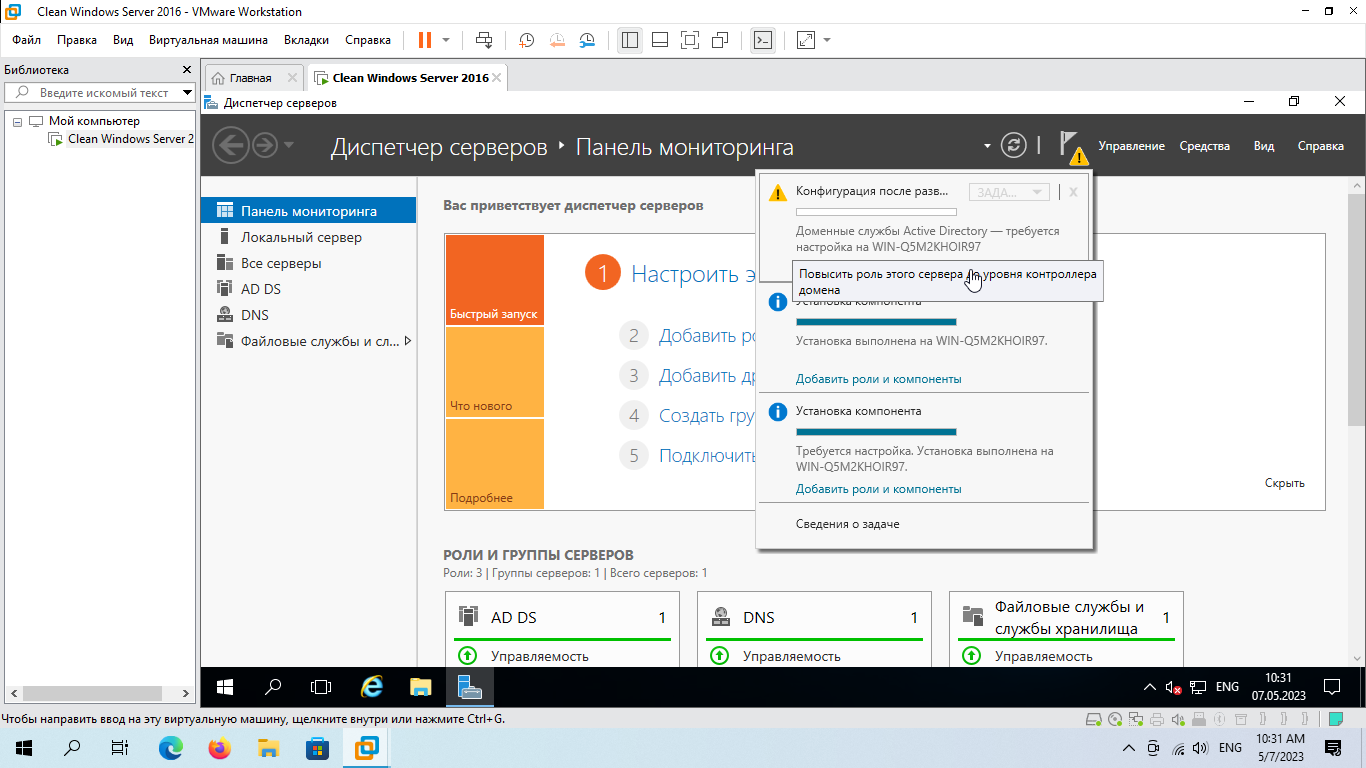
\includegraphics[width=0.85\textwidth]{9_0051}
    \caption{Начинаем процесс повышения роли этого сервера до уровня контроллера домена}
    \label{img:0051}
  \end{figure}

  \begin{figure}[H]
    \centering
    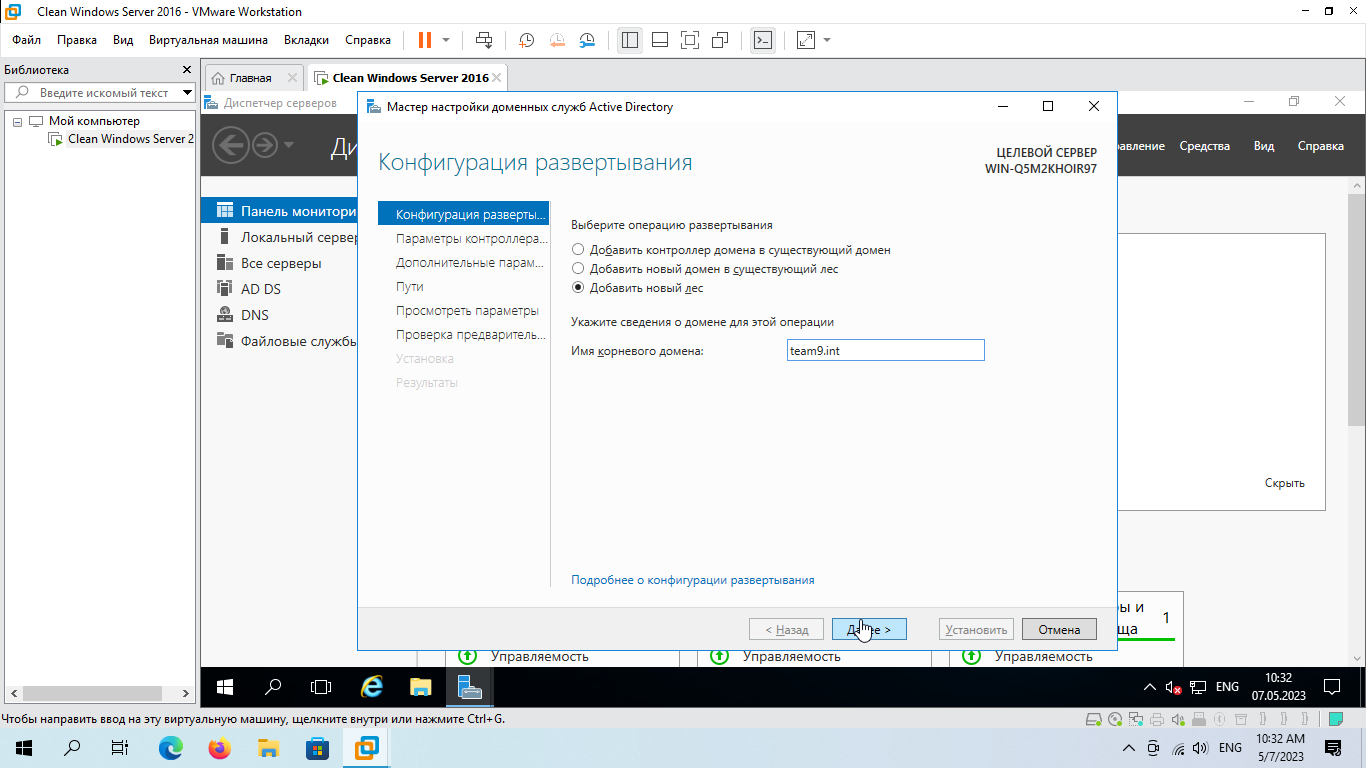
\includegraphics[width=0.85\textwidth]{9_0052}
    \caption{Указываем имя домена}
    \label{img:0052}
  \end{figure}

  Имя домена было выбрано в соответствии с указаниями к 9 варианту - team9.int.

  \begin{figure}[H]
    \centering
    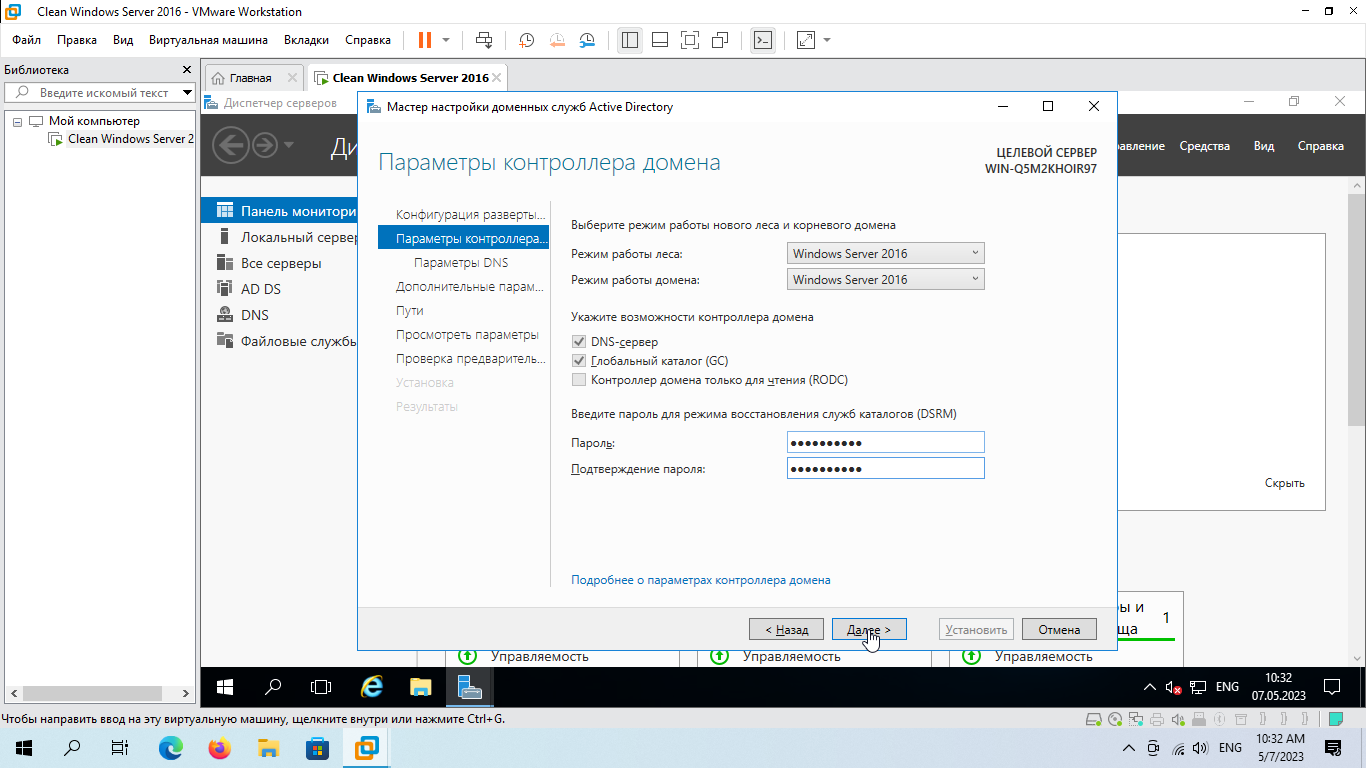
\includegraphics[width=0.85\textwidth]{9_0053}
    \caption{Указываем пароль}
    \label{img:0053}
  \end{figure}

  \begin{figure}[H]
    \centering
    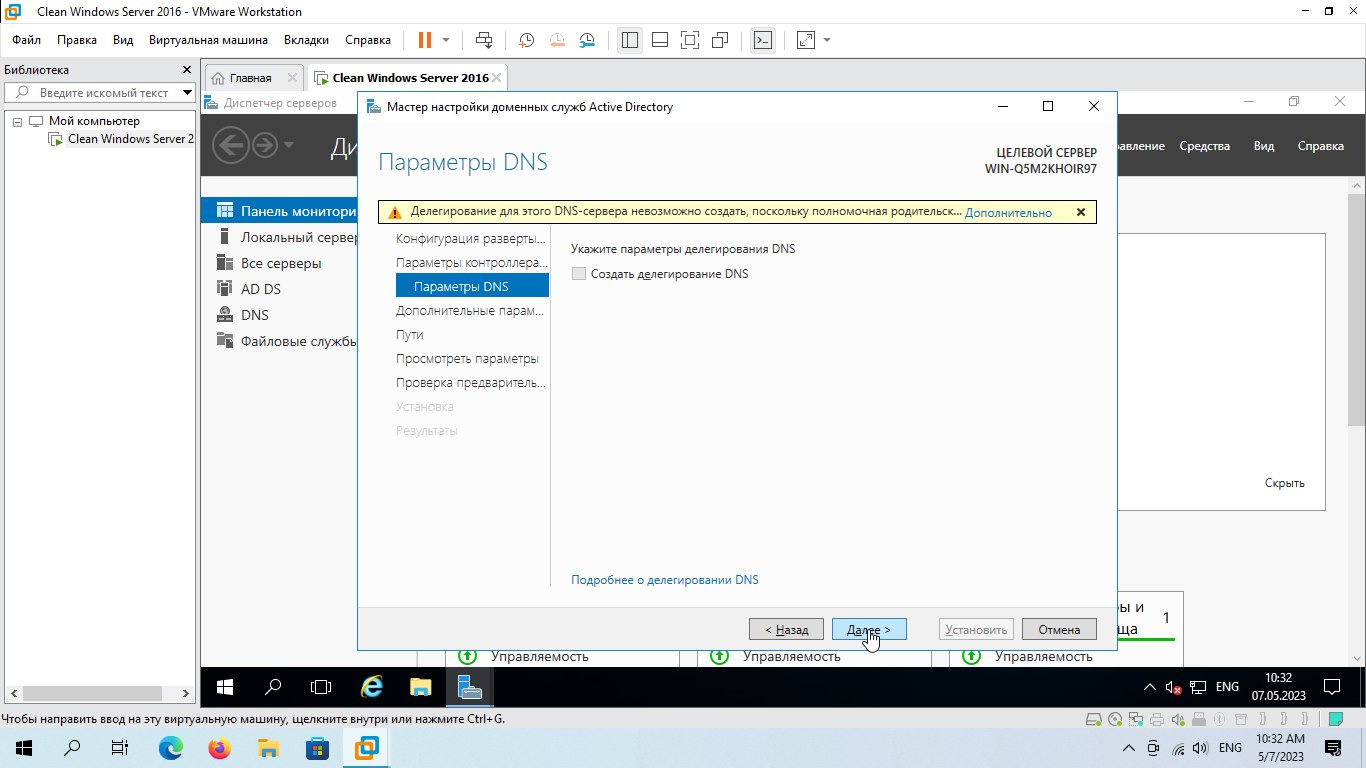
\includegraphics[width=0.85\textwidth]{9_0054}
    \caption{Далее}
    \label{img:0054}
  \end{figure}

  \begin{figure}[H]
    \centering
    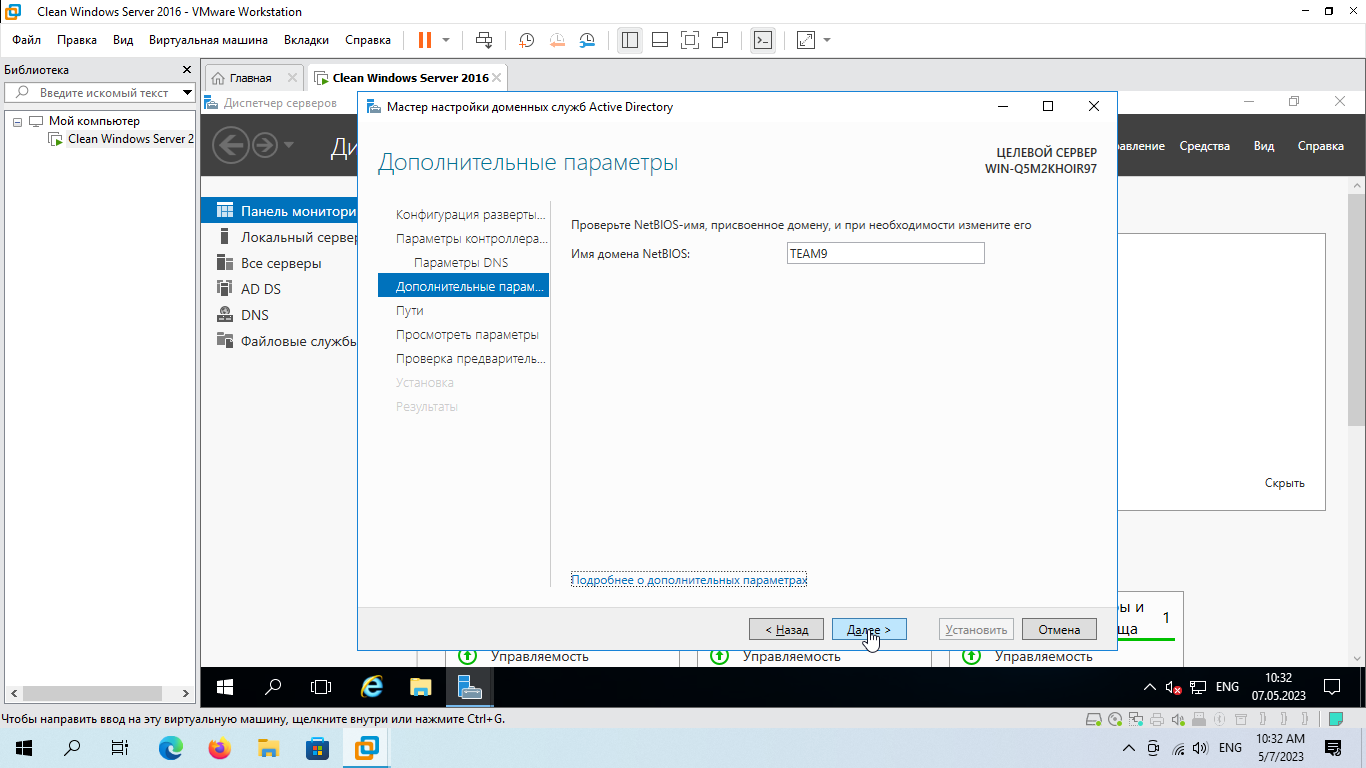
\includegraphics[width=0.85\textwidth]{9_0055}
    \caption{Имя домена \textit{NetBIOS} установилось автоматически}
    \label{img:0055}
  \end{figure}

  \begin{figure}[H]
    \centering
    \includegraphics[width=0.85\textwidth]{9_0056}
    \caption{Пути не изменяем}
    \label{img:0056}
  \end{figure}

  \begin{figure}[H]
    \centering
    \includegraphics[width=0.85\textwidth]{9_0057}
    \caption{Далее}
    \label{img:0057}
  \end{figure}

  \begin{figure}[H]
    \centering
    \includegraphics[width=0.85\textwidth]{9_0058}
    \caption{Далее}
    \label{img:0058}
  \end{figure}

  \begin{figure}[H]
    \centering
    \includegraphics[width=0.85\textwidth]{9_0059}
    \caption{Установка завершена - требуется перезагрузка}
    \label{img:0059}
  \end{figure}

  \begin{figure}[H]
    \centering
    \includegraphics[width=0.85\textwidth]{9_0060}
    \caption{Перезагрузка}
    \label{img:0060}
  \end{figure}

  \begin{figure}[H]
    \centering
    \includegraphics[width=0.85\textwidth]{9_0062}
    \caption{Входим в учетную запись пользователя}
    \label{img:0062}
  \end{figure}

  Теперь домен создан и настроен, можно переходить к конфигурированию \textit{DNS} сервера.

  \subsection{Настройка \textit{DNS} сервера}

  \begin{figure}[H]
    \centering
    \includegraphics[width=0.85\textwidth]{9_0063}
    \caption{Выбираем \textit{DNS} в списке средств}
    \label{img:0063}
  \end{figure}

  \begin{figure}[H]
    \centering
    \includegraphics[width=0.85\textwidth]{9_0065}
    \caption{Только что созданные и запущенный \textit{DNS} сервер в зоне прямого просмотра}
    \label{img:0065}
  \end{figure}

  \subsubsection{Создание зон}

  \begin{figure}[H]
    \centering
    \includegraphics[width=0.85\textwidth]{9_0066}
    \caption{Создадим новую зону прямого просмотра}
    \label{img:0066}
  \end{figure}

  \begin{figure}[H]
    \centering
    \includegraphics[width=0.85\textwidth]{9_0067}
    \caption{Запущен мастер создания зоны}
    \label{img:0067}
  \end{figure}

  \begin{figure}[H]
    \centering
    \includegraphics[width=0.85\textwidth]{9_0068}
    \caption{Указываем тип зоны - основная}
    \label{img:0068}
  \end{figure}

  \begin{figure}[H]
    \centering
    \includegraphics[width=0.85\textwidth]{9_0069}
    \caption{Указываем репликацию зоны - на весь домен}
    \label{img:0069}
  \end{figure}

  \begin{figure}[H]
    \centering
    \includegraphics[width=0.85\textwidth]{9_0073}
    \caption{Указываем имя зоны}
    \label{img:0073}
  \end{figure}

  В методичке к лабораторной работы не было четких указаний к имени зоны, были
  только к \textbf{имени домена}, поэтому здесь \textit{team9.zone}.

  \begin{figure}[H]
    \centering
    \includegraphics[width=0.85\textwidth]{9_0074}
    \caption{Разрешаем безопасные динамические обновления}
    \label{img:0074}
  \end{figure}

  \begin{figure}[H]
    \centering
    \includegraphics[width=0.85\textwidth]{9_0075}
    \caption{Готово}
    \label{img:0075}
  \end{figure}

  \begin{figure}[H]
    \centering
    \includegraphics[width=0.85\textwidth]{9_0076}
    \caption{Зона создана и уже в состоянии "Выполняется"}
    \label{img:0076}
  \end{figure}

  \begin{figure}[H]
    \centering
    \includegraphics[width=0.85\textwidth]{9_0077}
    \caption{Аналогично создадим зону обратного просмотра}
    \label{img:0077}
  \end{figure}

  \begin{figure}[H]
    \centering
    \includegraphics[width=0.85\textwidth]{9_0078}
    \caption{Далее}
    \label{img:0078}
  \end{figure}

  \begin{figure}[H]
    \centering
    \includegraphics[width=0.85\textwidth]{9_0079}
    \caption{Тип зоны - основная}
    \label{img:0079}
  \end{figure}

  \begin{figure}[H]
    \centering
    \includegraphics[width=0.85\textwidth]{9_0080}
    \caption{Область репликации - весь домен}
    \label{img:0080}
  \end{figure}

  \begin{figure}[H]
    \centering
    \includegraphics[width=0.85\textwidth]{9_0081}
    \caption{Настроим зону для работы с \textit{IPv4} адресами}
    \label{img:0081}
  \end{figure}

  \begin{figure}[H]
    \centering
    \includegraphics[width=0.85\textwidth]{9_0082}
    \caption{Указываем адрес сети - 192.168.142.0}
    \label{img:0082}
  \end{figure}

  \begin{figure}[H]
    \centering
    \includegraphics[width=0.85\textwidth]{9_0083}
    \caption{Разрешаем безопасные динамические обновления}
    \label{img:0083}
  \end{figure}

  \begin{figure}[H]
    \centering
    \includegraphics[width=0.85\textwidth]{9_0084}
    \caption{Готово - зона обратного просмотра создана}
    \label{img:0084}
  \end{figure}

  \subsubsection{Создание узлов}

  Создадим в зоне прямого просмотра узел, ссылающийся на адрес текущего компьютера
  (сервера, 192.168.142.2):

  \begin{figure}[H]
    \centering
    \includegraphics[width=0.85\textwidth]{9_0085}
    \caption{Начинаем создание A узла}
    \label{img:0085}
  \end{figure}

  \begin{figure}[H]
    \centering
    \includegraphics[width=0.85\textwidth]{9_0086}
    \caption{Указываем имя и адрес}
    \label{img:0086}
  \end{figure}

  Имя узла выбрано в соответствии с 9 вариантом - team9\textunderscore point.
  Также важно отметить галочку на создании \textit{PTR} записи.

  \begin{figure}[H]
    \centering
    \includegraphics[width=0.85\textwidth]{9_0087}
    \caption{Узел добавлен и готов к работе}
    \label{img:0087}
  \end{figure}

  \textit{Использование настроенного \textit{DNS} сервера}

   Теперь сделаем так, чтобы сам сервера (текущий компьютер) обращался
   к себе же самому для того, чтобы выполнить какой-либо \textit{DNS} запрос
   (назначим его самого его же предпочтительным \textit{DNS} сервером).

   Для начала проверим при помощи \textit{ipconfig}, какой \textit{DNS}
   сервер используется сейчас:

  \begin{figure}[H]
    \centering
    \includegraphics[width=0.85\textwidth]{9_0089}
    \caption{Результат работы \textit{ipconfig}}
    \label{img:0089}
  \end{figure}

  Видно, что в качестве \textit{DNS} сервера указан \textit{localhost},
  то есть сам же компьютер, что как раз и соответсвует необходимым настройкам.
  Скорее всего, операционная система сама внесла необходимые изменения
  после установки роли \textit{DNS} сервера.

  Проверим, как работают только что настроенные узлы:

  \begin{figure}[H]
    \centering
    \includegraphics[width=0.85\textwidth]{9_0090}
    \caption{Выполняем \textit{DNS} запросы при помощи \textit{nslookup}}
    \label{img:0090}
  \end{figure}

  Первый запрос показывает, что на используемом \textit{DNS} сервере есть
  запись, которая к имени \textit{team9\textunderscore point.team9.zone} ставит в 
  соответсвии \textit{IPv4} адрес 192.168.142.2 - все как и было настроено.

  Второй запрос показывает, что работает и определение внешних (не принадлежащих
  домену) адресов, однако такая функциональность пока не была настроена -
  посмотрим свойства текущего \textit{DNS} сервера:

  \begin{figure}[H]
    \centering
    \includegraphics[width=0.85\textwidth]{9_0093}
    \caption{Открываем свойства сервера}
    \label{img:0093}
  \end{figure}

  \begin{figure}[H]
    \centering
    \includegraphics[width=0.85\textwidth]{9_0094}
    \caption{Вкладка "Сервер пересылки"}
    \label{img:0094}
  \end{figure}

  Видно, что адрес \textit{DNS} сервера, который был указан при конфигурировании
  сетевого адаптера автоматически добавиося в список адресов пересылки, то есть
  если на текущий сервер придет \textit{DNS} запрос, который он не сможет
  обработать самостоятельно, он отправит его на 192.168.142.1.

  Добавим еще один адрес пересылки:

  \begin{figure}[H]
    \centering
    \includegraphics[width=0.85\textwidth]{9_0095}
    \caption{Нажимаем кнопку "Изменить"}
    \label{img:0095}
  \end{figure}

  \begin{figure}[H]
    \centering
    \includegraphics[width=0.85\textwidth]{9_0096}
    \caption{Добавляем 8.8.8.8 - адрес Google DNS}
    \label{img:0096}
  \end{figure}

  \begin{figure}[H]
    \centering
    \includegraphics[width=0.85\textwidth]{9_0098}
    \caption{Готово}
    \label{img:0098}
  \end{figure}

  \begin{figure}[H]
    \centering
    \includegraphics[width=0.85\textwidth]{9_0100}
    \caption{Еще раз проверяем, что все работает}
    \label{img:0100}
  \end{figure}

  \section{Вопросы по заданию}

  \begin{enumerate}
    \item {
      \textbf{Зачем нужна запись типа AAAA}

      Данная запись предназначена для работы с \textit{IPv6} адресами (в отличие от
      A записи, которая работает с \textit{IPv4}).
    }
    \item {
      \textbf{Зачем нужна зона обратного просмотра}

      Зона прямого просмотра ставит буквенному имени в соответсвтвие численный \textit{IP}
      адрес, что позволяет быстро узнавать адрес сервера, но не позволяет узнать к какому
      имени принадлежит какой-то \textit{IP} адрес.

      Для этой задачи служит зона обратного просмотра, она позволяет быстро определить
      к какому имени принадлежит \textit{IP} адрес.
    }
    \item {
      \textbf{Как проверить запись зоны обратного просомтра}

      Выполнить \textit{DNS} запрос записи типа \textit{PTR} (PoinTer Record) (можно
      выполнить в том числе и через nslookup).
    }
    \item {
      \textbf{Зачем нужна запись типа MX}

      \textbf{M}ail \textbf{E}change записи используются для хранения \textit{IP}
      адресов почтовых серверов (в частности работающих по протоколу \textit{SMTP}).

      Пример: для того, чтобы отправить email на konstantimp@yandex.ru, не получиться
      отправить его по \textit{SMTP} на адрес, который будет получен при запросе A
      записи для yandex.ru.
    }
    \item {
      \textbf{Зачем нужна запись типа NS}

      Запись NS (NameServer) определяет авторитетные серверы имен для домена. Авторитетные серверы имен - это серверы, которые используются для разрешения запросов к именам хостов и определения того, какие IP-адреса следует использовать для доступа к данному серверу.
    }
    \item {
      \textbf{Какой командой в системе Windows можно проверить DNS запись на удаленном сервере}

      \begin{minted}{bash}
        nslookup
      \end{minted}
    }
    \item {
      \textbf{Приведите пример команды для получения записей всех типов для доменного имени hse.ru}

      \begin{minted}{bash}
        nslookup -type=any hse.ru
      \end{minted}
    }
  \end{enumerate}

  \section{Вывод}

  В ходе данной работы мне удалось познакомиться с прицнипом работы \textit{DNS},
  самостоятельно его настроить и протестировать.

\end{document}
